\documentclass[11pt]{article}

	\usepackage{apacite}
	\usepackage{epsfig}
	\usepackage{bm}

	\evensidemargin=0cm
	\oddsidemargin=0cm
	\topmargin=0cm
	\textwidth=16cm
	\textheight=22cm
	\raggedbottom

	\hyphenation{stoch-as-tic}
	\renewcommand{\arraystretch}{1}

	\newcommand{\condon}{|}
	\newcommand{\vctr}[1]{\bm{#1}}
	\newcommand{\panel}[1]{#1}
	\newcommand{\gp}{g}
	\newcommand{\dnorm}{\mathcal{Z}}
	\newcommand{\bfc}{}
	\newcommand{\efc}{\vspace*{15pt}}
	\newcommand{\fcs}{}
	\newcommand{\acs}{}
	\newcommand{\tbsp}{\vspace*{0pt}}
	\newcommand{\cnt}{z}
	\newcommand{\HH}{\mathcal{H}}

	\newcommand{\presec}{}
	\newcommand{\postsec}{}
	\newcommand{\capspace}{}

% ---------- watermark -----------
\usepackage[firstpage]{draftwatermark}
\SetWatermarkAngle{0}
\SetWatermarkFontSize{0.25cm}
\SetWatermarkVerCenter{0.75cm}
\SetWatermarkLightness{0.5}
\SetWatermarkHorCenter{14cm}
\SetWatermarkText{\shortstack[l]{
Navarro, D. J. and Griffiths, T. L. (2008). Latent features in similarity judgments:\\
A nonparametric Bayesian approach. Neural Computation, 20, 2597-2628. \\
http://dx.doi.org/10.1162/neco.2008.04-07-504
}}
\SetWatermarkScale{1}
% -------------------------------

	\title{Latent features in similarity judgments:\\ A nonparametric Bayesian approach}
	\author{Danielle J. Navarro  \\
	School of Psychology  \\
	University of Adelaide \\ \\
	Thomas L. Griffiths \\
	Department of Psychology \\
	University of California, Berkeley}
	\pagestyle{myheadings}
	\markboth{Bayesian Additive Clustering}{Bayesian Additive Clustering}
	\date{}


\begin{document}
\maketitle
%\setlength{\baselineskip}{24pt}

\begin{abstract}\noindent
%\setlength{\baselineskip}{24pt}
One of the central problems in cognitive science is determining the mental representations that underlie human inferences. Solutions to this problem often rely on the analysis of subjective similarity judgments, on the assumption that recognizing ``likenesses'' between people, objects and events is crucial to everyday inference. One such solution is provided by the additive clustering model, which is widely used to infer the features of a set of stimuli from their similarities, on the assumption that similarity is a weighted linear function of common features. Existing approaches for implementing additive clustering often lack a complete framework for statistical inference, particularly with respect to choosing the number of features. To address these problems, this paper develops a fully Bayesian formulation of the additive clustering model, using methods from nonparametric Bayesian statistics to allow the number of features to vary. We use this to explore several approaches to parameter estimation, showing that the nonparametric Bayesian approach provides a straightforward way to obtain estimates of both the number of features and their importance.
\end{abstract}
\newpage

\presec \section{Introduction} \postsec

One of the central problems in cognitive science is determining the mental representations that underlie human inferences. A variety of solutions to this problem are based on the analysis of subjective similarity judgments, on the assumption that recognizing ``likenesses'' between people, objects and events is crucial to everyday inference. However, since subjective similarity cannot be derived from a straightforward analysis of objective stimulus characteristics \cite{goodman72}, it is important that mental representations be constrained by empirical data \cite{komatsu92,lee98}. By defining a probabilistic model that accounts for the similarity between stimuli based on their representation, statistical methods can be used to infer these underlying representations from human judgments. The particular methods used to infer representions from similarity judgments depend on the nature of the underlying representations. For stimuli that are assumed to be represented as points in some psychological space, multidimensional scaling algorithms \cite{torgerson58} can be used to translate similarity judgments into stimulus locations. For stimuli that are assumed to be represented in terms of a set of latent features \cite{tversky77}, the {\em additive clustering} technique developed by \citeA{sheparda79} is the method of choice.

Additive clustering provides a method of assigning a set of latent features to a collection of objects, based on the observable similarities between those items. The model is related to factor analysis, multidimensional scaling and latent class models, and shares a number of important issues. When extracting a set of latent features we need to infer the dimension of the model (i.e., number of features), determine the best feature allocations, and estimate the saliency (or importance) weights associated with each feature. Motivated in part by these issues, this paper develops a fully Bayesian formulation of the additive clustering model, using methods from nonparametric Bayesian statistics to allow the number of features to vary. We use this to explore several approaches to parameter estimation, showing that the nonparametric Bayesian approach provides a straightforward way to obtain estimates of both the number of features and their importance.

In what follows, we assume that the data take the form of an $n \times n$ similarity matrix $\mathbf{S}=\left[s_{ij}\right]$, where $s_{ij}$ is the judged similarity between the $i$th and $j$th of $n$ objects. The various similarities are assumed to be symmetric (with $s_{ij}=s_{ji}$) and non-negative, often constrained to lie on the interval $\left[0, 1\right]$. It is also typical to assume that self-similarities $s_{ii}$ take on maximal values, and are generally not explicitly modeled. The source of such data can vary considerably: in psychology alone, similarity data have been collected using a number of experimental methodologies, including rating scales \cite<e.g.,>{kruschke93}, confusion probabilities \cite<e.g.,>{shepard72}, sorting tasks \cite<e.g.,>{rosenbergk75}, or forced-choice tasks \cite<e.g.,>{navarrol02}. Additionally, in applications outside psychology similarity matrices are often calculated using aspects of the objective structure of the stimulus items \cite<e.g.,>{dayhoff78,henikoff92}.


\presec \section{Latent Variable Models for Similarity Judgment} \postsec

The analysis of similarities is perhaps best treated as a question of inferring a {\it latent structure} from the observed similarity data, for which a variety of methods have been proposed. For instance, besides the latent features approach, latent metric spaces have been found using multidimensional scaling,  latent classes found by partitioning, and  latent trees constructed using hierarchical clustering and related methods. Even the factor analysis model for the analysis of covariances has been used for this purpose. Since additive clustering has close ties to these methods, we provide a brief overview.

{\it Multidimensional scaling.} The first method to be developed explicitly for the extraction of latent structure in similarity data was multidimensional scaling \cite{torgerson58,attneave50,shepard62,kruskal64a,kruskal64b,youngh38}, in which items are assumed to be represented as points in a low dimensional space, usually equipped with one of the Minkowski distance metrics \cite{minkowski1891}. The motivation behind this approach comes from measurement theory, with particular reference to psychophysical measurement \cite<e.g.,>{stevens46,stevens51}. In psychophysical scaling, the goal is to construct a latent  scale that translates a physical measurement (e.g., frequency) into a subjective state (e.g., pitch). Typically, however, stimuli may vary simultaneously in multiple respects, so the single scale generalizes to a latent metric space in which observed stimuli are located. Although multidimensional scaling is not always formalized as a statistical model, it is common to use squared error as a loss function, which agrees with the Gaussian error model adopted by some authors  \cite<e.g.,>{lee01}.

{\it Factor analysis.} The well-known factor analysis model (\citeNP{thurstone47}; see also \citeNP{spearman04,spearman27}) and the closely-related principal component analysis technique (\citeNP{pearson1901,hotelling33}; in effect the same model, minus the error theory - see \citeNP{lawleym63}) both predate multidimensional scaling by some years. In these approaches stimulus items are assumed to ``load'' on a set of latent variables or ``factors''. Since these variables are continuous-valued, factor analysis is closely related to multidimensional scaling. However, the ``common factors'' model makes different assumptions about similarity to the Minkowski distance metrics, so the two are not equivalent. Historically, neither factor analysis nor principal components were widely used for modeling similarity \cite<but see>{ekman54,ekman63}. In recent years this has changed somewhat, with principal components analysis becoming a standard method for making predictions about document similarities, under the name of ``latent semantic analysis'' \cite{landauerd97}. On occasions, those predictions have been compared to human similarity judgments \cite{leepw05}.

{\it Partitions.} A discrete alternative to the continuous methods provided by multidimensional scaling and factor analysis is clustering. The aim behind clustering is the unsupervised extraction of a classification system for different items, such that similar items tend to be assigned to the same class \cite{sokal74}. Clustering methods vary extensively \cite{jainmf99}, with different models imposing different structural constraints on how objects can be grouped, as illustrated in Figure \ref{MDLclustertypes}.  The {\it partitioning approach}, very commonly used as a general data analysis technique,  forces each object to be assigned to exactly one cluster.  This approach can be interpreted as grouping the objects into equivalence classes without specifying how the clusters relate to each other. For example, if the objects $A$ though $H$ in Figure \ref{MDLclustertypes}(a) correspond to people, the partition might indicate which of four different companies employs each person. Commonly-used methods for extracting partitions include heuristic methods such as $k$-means \cite{mcqueen67,hartiganw79}, as well as more statistically-motivated approaches based on mixture models \cite{wolfe70,mclachlanb88,kontkanenmbrt05}. Partitioning models are rarely used for the representation of stimulus similarities, though they are quite common for representing the similarities between people, sometimes in conjunction with the use of other models for representing stimulus similarities \cite<e.g.,>{mcadams95}.

{\it Hierarchies.} The major problem with partitioning models is that, in the example above, the representation does not allow a person to work for more than one company, and does not convey information about how the companies themselves are related. Other clustering schemes allow objects to belong to multiple classes. The hierarchical approach \cite{sneath57,sokals63,johnson67,dandrade78} allows for nested clusters, for instance.  Thus the arrangement in Figure \ref{MDLclustertypes}(b) could show not just the company employing each person, but also the division they work in within that company, and further subdivisions in the organizational structure. Useful extensions to this approach are provided by the additive tree \cite{buneman71,sattatht77}, extended tree \cite{cortert86} and bidirectional tree \cite{cunningham78} models.

\begin{figure*}
\begin{center}
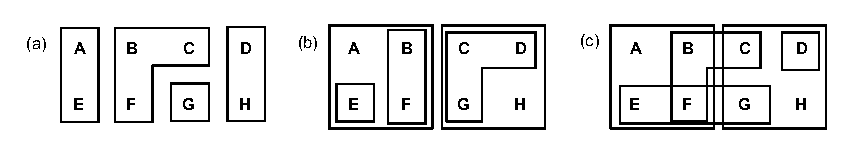
\epsfig{file=NECO-04-07-504-Figure1.eps, width=16cm}
\caption{\capspace Three different representational assumptions for clustering models, showing (a) partitioning, (b) hierarchical, and (c) overlapping structures.}
\label{MDLclustertypes}
\end{center}
\end{figure*}

\presec \section{Additive Clustering: A Latent Feature Model } \postsec

The additive clustering (ADCLUS) model \cite{sheparda79} was developed to provide a discrete alternative to multidimensional scaling, allowing similarity models to encompass a range of data sets for which spatial models seem inappropriate \cite{tversky77}. It provides a natural extension of the partitioning and hierarchical clustering models, and has an interpretation as a form of binary factor analysis. Viewed as a clustering technique, additive clustering is an example of {\it overlapping clustering} \cite{jardines68,colew70}, which imposes no representational restrictions on the clusters, allowing any cluster to include any object and any object to belong to any cluster \cite<e.g.,>[p. 88]{hutchinsonm97}. By removing these restrictions, overlapping clustering models can be interpreted as assigning features to objects.  For example, in Figure \ref{MDLclustertypes}(c), the five clusters could correspond to features like the company a person works for, the division they work in, the football team they support, their nationality, and so on. It is possible for two people in different companies to support the same football team, or have the same nationality, or have any other pattern of shared features. This representational flexibility allows overlapping clustering to be applied far more broadly than hierarchical clustering or partitioning methods.

Additive clustering relies on the {\it common features} measure for item similarities \cite{tversky77,navarrol04}, in which the empirically observed similarity $s_{ij}$ between items $i$ and $j$ is assumed to be well-approximated by a weighted linear function $\mu_{ij}$ of the features shared by the two items,
\begin{equation}
   \mu_{ij} = \sum_{k=1}^{m} w_k f_{ik} f_{jk}.
\end{equation}
In this expression, $f_{ik}=1$ if the $i$th object possesses the $k$th feature, and $f_{ik}=0$ if it does not, and $w_{k}$ is the non-negative saliency weight applied to that feature. Under these assumptions, a representation that uses $m$ common features to describe $n$ objects is defined by the $n \times m$ feature matrix $\mathbf{F}=\left[f_{ik}\right]$, and the saliency vector $\mathbf{w}=\left(w_1,\ldots,w_m\right)$. Accordingly, additive clustering techniques aim to uncover a feature matrix and saliency vector that provide a good approximation to the empirical similarities. In most applications it is assumed that there is a fixed ``additive constant'', a required feature possessed by all objects. It should be noted that the common features model upon which additive clustering is based has some shortcomings, since it disregards the influence of characteristics possessed by one item and not by the other (i.e., distinctive features), and is unable to accommodate continuously-varying properties. For this reason, a number of models have been developed that address these shortcomings \cite<e.g.>{navarro03,navarrol03,navarrol04}. Although this paper concentrates on the original additive clustering model, the approach could be naturally extended to accommodate these richer models.


To formalize additive clustering as a statistical model, it has become standard practice \cite{tenenbaum96,lee02b} to assume that the empirically observed similarities are drawn from a normal distribution with common variance $\sigma^2$, and means described by the common features model (more detailed suggestions are discussed by \citeNP{ramsay82}). Given the latent featural model $(\mathbf{F},\mathbf{w})$, we may write
  \begin{equation}
   \begin{array}{rclcl}
   s_{ij} &\condon & \mathbf{F},\mathbf{w},\sigma &\sim &\mbox{Gaussian}(\mu_{ij},\sigma^2). \\
   \end{array}
   \label{likelihoodmodel}
   \end{equation}
Note that $\sigma$ is a ``nuisance parameter'' in this model, denoting the amount of noise in the data. It provides a measure of the degree of precision of the experimental procedure, but does not convey information regarding the content of the latent mental representations that the experiment seeks to uncover. The statistical formulation of the model allows us to obtain the additive clustering decomposition of the similarity matrix,
   \begin{equation}
   \mathbf{S} = \mathbf{F}\mathbf{W}\mathbf{F}^\prime + \mathbf{E}, \label{adclus}
   \end{equation}
where $\mathbf{W}=\mbox{diag}(\mathbf{w})$ is a diagonal matrix with nonzero elements corresponding to the saliency weights, and $\mathbf{E}=[\epsilon_{ij}]$ is an $n \times n$ matrix with entries drawn from a Gaussian$(0,\sigma^2)$ distribution. This is illustrated in Figure~\ref{adclusdecomp}, which decomposes a continuously varying similarity matrix $\mathbf{S}$ into the binary feature matrix $\mathbf{F}$, non-negative weights $\mathbf{W}$, and error terms $\mathbf{E}$.

\begin{figure*}
\begin{center}
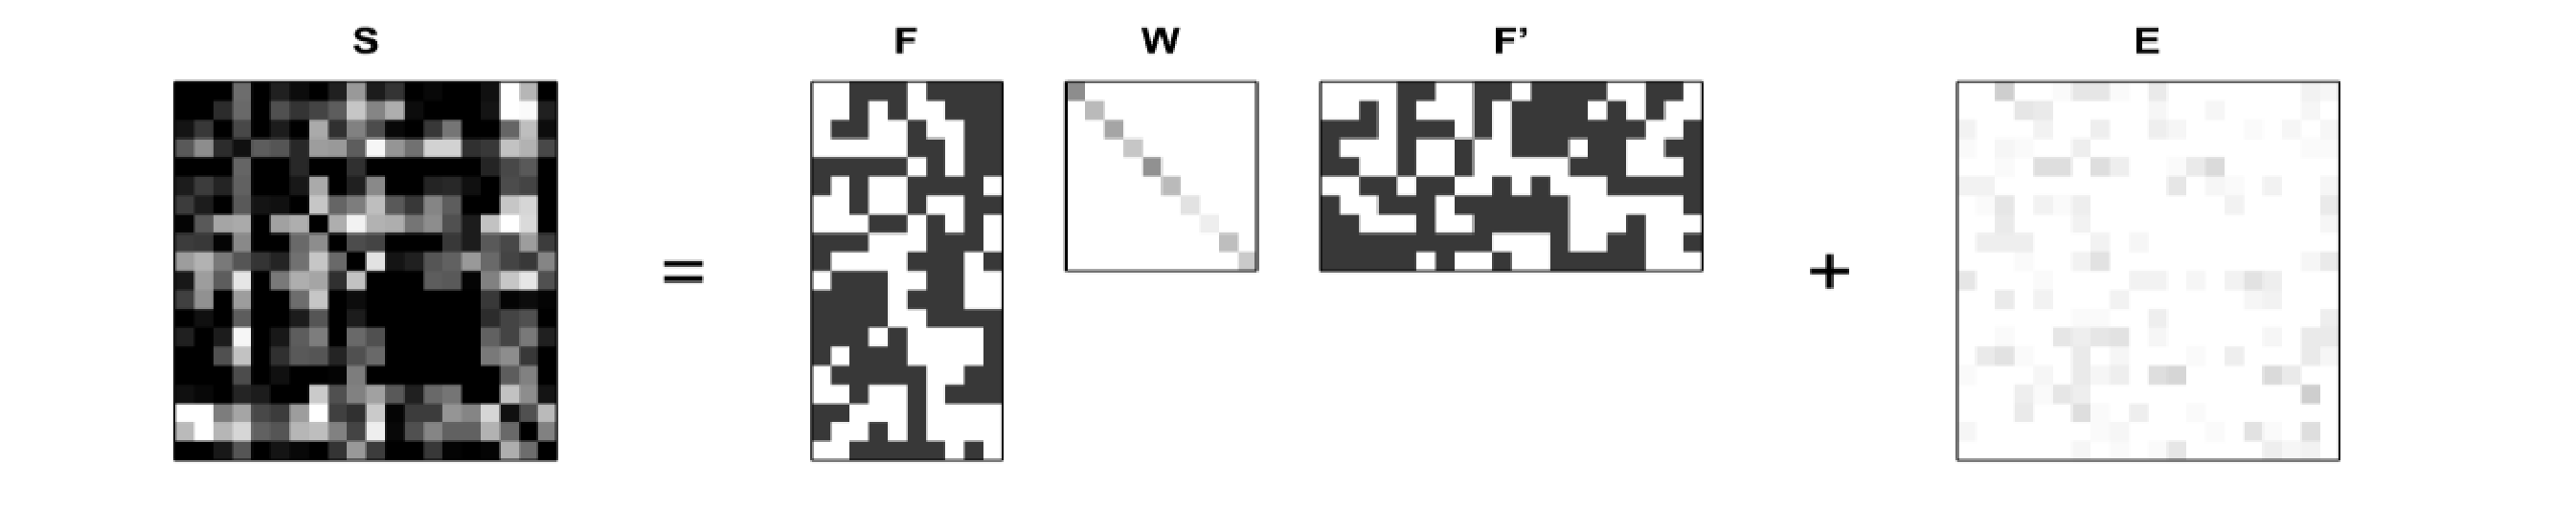
\epsfig{file=NECO-04-07-504-Figure2.eps, width=16cm}
\caption{\capspace The additive clustering decomposition of a similarity matrix. A continuously varying similarity matrix $\mathbf{S}$ may be decomposed into a binary feature matrix $\mathbf{F}$, a diagonal matrix of non-negative weights $\mathbf{W}$, and a matrix of error terms $\mathbf{E}$.\efc}
\label{adclusdecomp}
\end{center}
\end{figure*}

Additive clustering also has a factor analytic interpretation \cite{sheparda79,mirkin87}, since Equation~\ref{adclus} has the same form as the factor analysis model, with the ``feature loadings'' $f_{ik}$ constrained to 0 or 1. By imposing this constraint, additive clustering enforces a variant of the ``simple structure'' concept \cite[ch. 14]{thurstone47} that provides the theoretical basis for many factor rotation methods currently in use \cite<see>{browne01}. To see this, it suffices to note that  the most important criterion for simple structure is {\it sparsity}. In the extreme case, illustrated in the top row of Figure~\ref{simple1}, each item might load only on a single factor, yielding a partition-like representation (panel a) of the item vectors (shown in panel b). As a consequence, the factor-loading vectors project onto a very constrained part of the unit sphere (panel c). Although most factor rotation methods seek to approximate this partition-like structure \cite[p. 116]{browne01}, Thurstone himself allowed more general patterns of sparse factor loadings. Figure~\ref{simple1}(d) provides an illustration, corresponding to a somewhat different configuration of items in the factor space (panel e) and on the unit sphere (panel f). The additive clustering model is similarly general in terms of the pattern of zeros it allows, as illustrated in Figure~\ref{adclusscheme}(a).  However, by forcing all ``loadings'' to be 0 or 1, every feature vector is constrained to lie at one of the vertices of the unit cube, as shown in Figure~\ref{adclusscheme}(b). When these vectors are projected down onto the unit sphere, they show a different, though clearly constrained pattern. It is in this sense that the additive clustering model implements the simple structure concept, and is the motivation behind the ``qualitative factor analysis'' view of additive clustering \cite{mirkin87}.

\presec \section{Existing Approaches to Additive Clustering}

Since the introduction of the additive clustering model, a range of algorithms have been used to infer features, including ``subset selection'' \cite{sheparda79}, expectation maximization \cite{tenenbaum96}, continuous approximations \cite{arabiec80} and stochastic hillclimbing \cite{lee02b} among others. A review, as well as an effective combinatorial search algorithm, is given by \citeA{ruml02}. However, in order to provide a context, we present a brief discussion of some of the existing approaches.

The original additive clustering technique \cite{sheparda79} was a combinatorial optimization algorithm that employed a heuristic method to reduce the space of possible cluster structures to be searched. Shepard and Arabie observed that a subset of the stimuli in the domain is most likely to constitute a feature if the pairwise similarities of the stimuli in the subset are high. They define the $s$-level of a set of items $c$, to be the lowest pairwise similarity rating for two stimuli within the subset. Further, the subset $c$ is {\it elevated} if and only if every larger subset that contains $c$ has a lower $s$-level than $c$. Having done so, they constructed the algorithm in two stages. In the first step, all elevated subsets are found. In the second step, the saliency weights are found and the set of included features is reduced. The weight initially assigned to each potential cluster is proportional to its {\it rise}, defined as the difference between the $s$-level of the subset and the minimum $s$-level of any subset containing the original subset. The weights are then iteratively adjusted by a gradient descent procedure.

The next major development in inference algorithms for the ADCLUS model was the introduction of a mathematical programming approach \cite{arabiec80}. In this technique, the discrete optimization problem is recast as a continuous one. The cluster membership matrix $\mathbf{F}$ is initially allowed to assume continuously varying values, rather than the binary membership values required in the final solution. An error function is defined as the weighted sum of two parts, the first being the sum squared error and the second being a penalty function designed to push the elements of $\mathbf{F}$ towards 0 or 1.

A statistically motivated approach proposed by \citeA{tenenbaum96} uses the expectation maximization (EM) algorithm \cite{dempsterlr77}. As with the mathematical programming formulation, the number of features needs to be specified in advance, and the discrete problem is (in effect) converted to a continuous one. The EM algorithm for additive clustering consists of an alternating two-step procedure. In the E-step, the saliency weights are held constant, the expected sum squared error is estimated, and (conditional on these saliency weights), the expected values for the elements of $\mathbf{F}$ are calculated. Then, using the expected values for the feature matrix calculated during the E-step, the M-step finds a new set of saliency weights that minimize the expected sum squared error. As the EM algorithm iterates, the value of $\sigma$ is reduced, and the expected assignment values converge to 0 or 1, yielding a final feature matrix $\mathbf{F}$ and saliency weights $\mathbf{w}$.

Note that the EM approach treates $\sigma$ as something more akin to a ``temperature'' parameter rather than a genuine element of the data-generating process. Moreover, it still requires the number of features to be fixed in advance. To redress some of these problems, \citeA{lee02b} proposed a simple stochastic hillclimbing algorithm that ``grows'' an additive clustering model. The algorithm initially specifies a single-feature representation, which is optimized by ``flipping'' the elements of $\mathbf{F}$ (i.e., $f_{ik} \rightarrow 1-f_{ik}$) one at a time, in a random order. Every time a new feature matrix is generated, best-fitting saliency weights $\mathbf{w}^{*}$ are found by solving the corresponding non-negative least squares problem \cite<see>{lawhan74}, and the solution is evaluated. Whenever a better solution is found, the flipping process restarts. If flipping $f_{ik}$ results in an inferior solution, it is flipped back. If no element of $\mathbf{F}$ can be flipped to provide a better solution, a local minimum has been reached. Since, as \citeA{tenenbaum96} observed, additive clustering tends to be plagued with local minima problems, the algorithm allows the locally optimal solution to be ``shaken'', by randomly flipping several elements of $\mathbf{F}$ and restarting, in order to find a globally optimal solution. Once this process terminates, a new (randomly generated) cluster is added, and this solution is used as the starting point for a new optimization procedure. Importantly, potential solutions are evaluated using the stochastic complexity measure \cite{rissanen96}, which provides a statistically-principled method for determining the number of features to include in the representation (and under some situations has a Bayesian interpretation; see \citeNP{myungbp00}).



\begin{figure*}
\begin{center}
\begin{tabular}{ccc}
\raisebox{2cm}{ \scriptsize \begin{tabular}{|ccc|}\hline  I & II & III \\ \hline x & 0&0\\ x &0 &0\\ x & 0& 0\\ 0& x&0 \\0 & x&0\\ 0&x&0 \\ 0& 0& x\\ 0& 0& x \\ 0& 0& x \\ \hline \end{tabular} } & 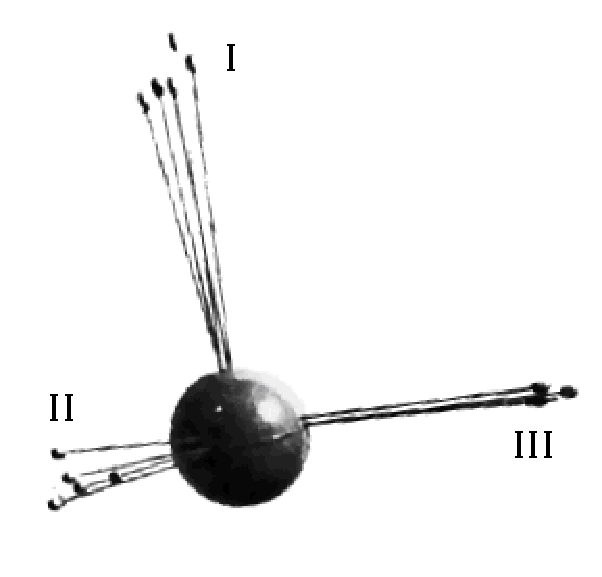
\epsfig{file=NECO-04-07-504-Figure3b.eps, width=4.5cm} & 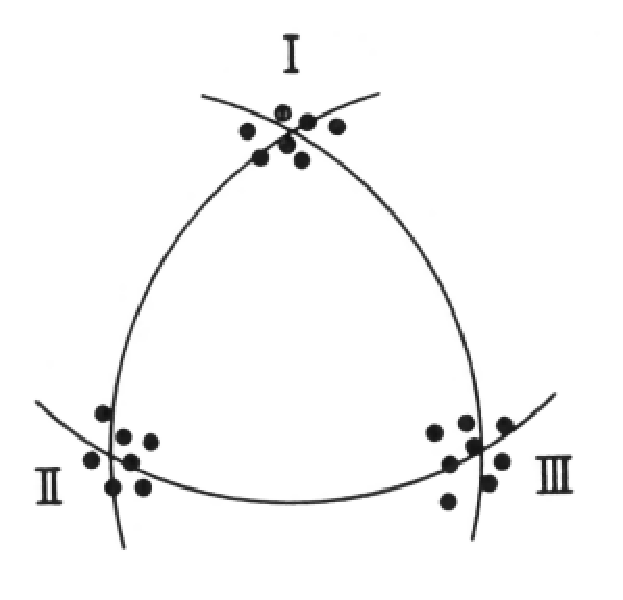
\epsfig{file=NECO-04-07-504-Figure3c.eps, width=4cm} \\ (a) & (b) & (c) \vspace*{10pt} \\
 \raisebox{2cm}{\scriptsize \begin{tabular}{|ccc|}\hline I & II & III \\ \hline x & 0&0\\ 0 & x&0\\ 0 & 0& x\\ x& x& 0\\x & x&0\\x & 0&x \\x & 0& x\\ 0 &x & x \\ 0&x & x \\ \hline \end{tabular} }  & 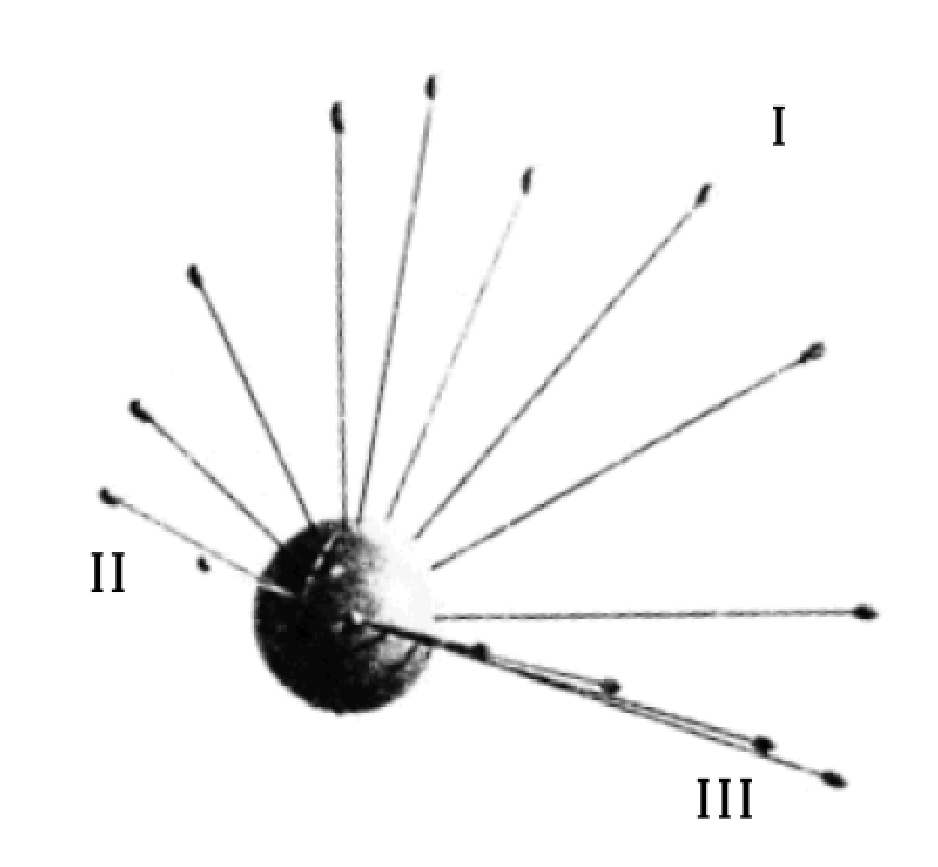
\epsfig{file=NECO-04-07-504-Figure3e.eps, width=4.75cm}
& 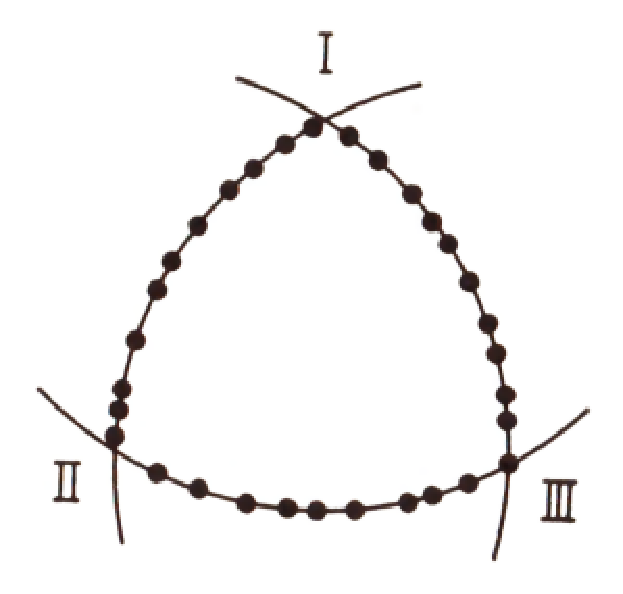
\epsfig{file=NECO-04-07-504-Figure3f.eps, width=4cm} \\ (d) & (e) & (f) \\
\end{tabular}
\caption{\capspace Simple structures in a three-factor solution, adapted from Thurstone's \protect\citeyear{thurstone47} original examples (p.126-127, 183-186). In the tables, crosses denote non-zero factor loadings. The middle panels illustrate possible item vectors in the solutions, and the right panels show corresponding projections onto the unit sphere. The partition-style solution shown in the top row (panels a-c) is the classic example of a simple structure, but more general sparse structures of the kind illustrated in the lower row (panels d-f) are allowed.\efc}
\label{simple1}
\end{center}
\end{figure*}


\begin{figure*}
\begin{center}
\begin{tabular}{ccc}
\raisebox{2cm}{\scriptsize \begin{tabular}{|ccc|}\hline I & II & III \\ \hline 1 & 0&0\\ 0 & 1&0\\ 0 &0 & 0\\ 0& 0& 1\\1 & 1&0\\1 & 0&1 \\1 & 0& 1\\  0&1 & 1 \\1& 1 & 1 \\ \hline \end{tabular} }  &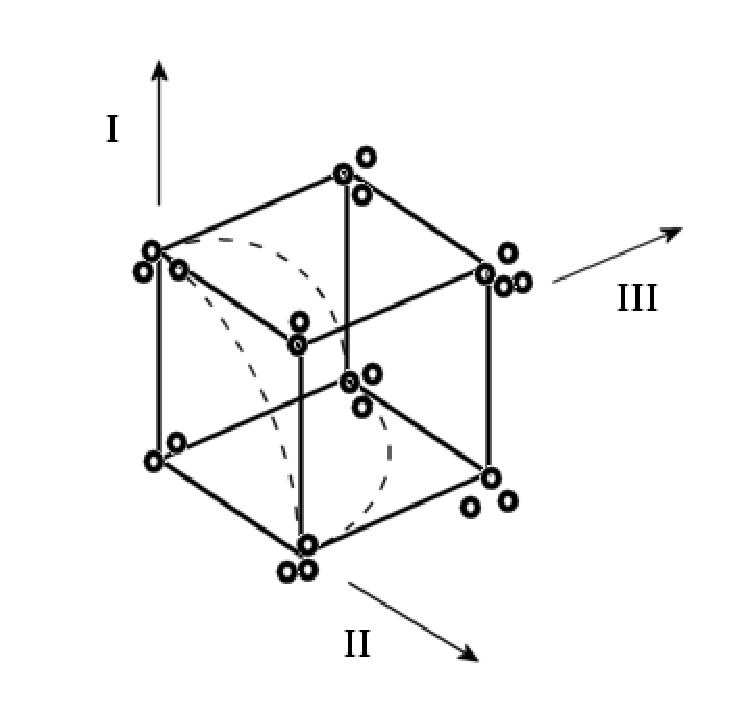
\epsfig{file=NECO-04-07-504-Figure4b.eps, width=4.75cm} & 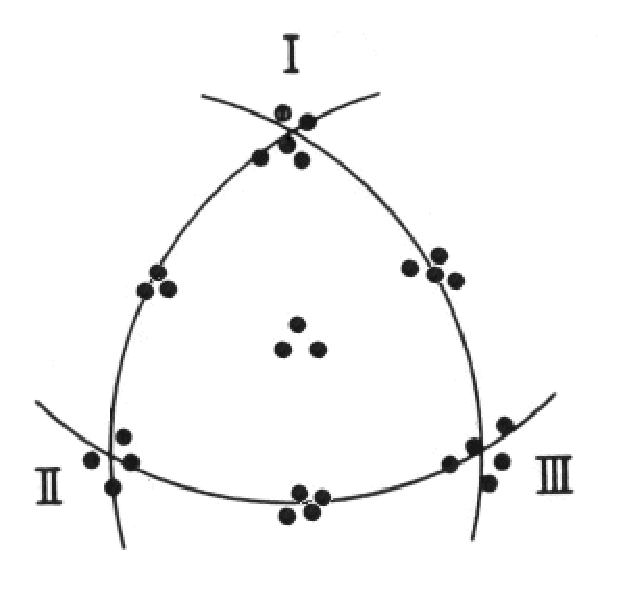
\epsfig{file=NECO-04-07-504-Figure4c.eps, width=4cm} \\ (a) & (b) & (c)
\end{tabular}
\caption{\capspace The variant of simple structure enforced by the ADCLUS model. Any sparse pattern of binary loadings is allowable (panel a), and the natural way to interpret item vectors is in terms of the vertices of the unit cube (panel b) on which all feature vectors lie, rather than project the vectors onto the unit sphere (panel c).\efc}
\label{adclusscheme}
\end{center}
\end{figure*}


\presec \section{A Nonparametric Bayesian ADCLUS Model} \postsec

The additive clustering model provides a method for relating a latent feature set to an observed similarity matrix. In order to complete the statistical framework, we need to specify a method for learning a feature set and saliency vector from data. In contrast to the approaches discussed in the previous section, our solution is to cast the additive clustering model in an explicitly Bayesian framework, placing priors over both $\mathbf{F}$ and $\mathbf{w}$, and then basing subsequent inferences on the full joint posterior distribution $p(\mathbf{F},\mathbf{w} \condon \mathbf{S})$ over possible representations in light of the observed similarities. However, since we wish to allow the additive clustering model the flexibility to extract a range of structures from the empirical similarities $\mathbf{S}$, we want the implied marginal prior $p(\mathbf{S})$ to have broad support. In short, we have a nonparametric problem, in which the goal is to learn from data without making any strong prior assumptions about the family of distributions that might best describe those data.

The rationale for adopting a nonparametric approach is that the generative process for a particular data set is unlikely to belong to any finite-dimensional parametric family, so it would be preferable to avoid making this false assumption at the outset. From a Bayesian perspective, nonparametric assumptions require us to place a prior distribution that has broad support across the space of probability distributions. In general, this is a hard problem: thus, to motivate a nonparametric prior for a latent feature model, it is useful to consider the simpler case of latent class models. In these models, a common choice relies on the Dirichlet process \cite{ferguson73}. The Dirichlet process is by far the most widely-used distribution in Bayesian nonparametrics, and specifies a distribution that has broad support across the discrete probability distributions. The distributions indexed by the Dirichlet process can be expressed as countably infinite mixtures of point masses \cite{sethuraman94}, making them ideally suited to act as priors in infinite mixture models \cite{escobarw95,rasmussen00}. For the current paper, however, it is more important to note that the Dirichlet process also implies a distribution over latent class assignments: any two observations in the sample that were generated from the same mixture component may be treated as members of the same class, allowing us to specify priors over infinite partitions. This implied prior can be useful for data clustering purposes \cite<e.g.,>{navarrogsl06}, particularly since samples from this prior can be generated using a simple stochastic process known as the {\it Chinese restaurant process}\footnote{The origin of the term is due to Jim Pitman and Lester Dubner, and refers to the Chinese restaurants in San Francisco that appear to have infinite seating capacity. The term ``Indian buffet process'' introduced later is named by analogy to the Chinese restaurant process.} \cite{blackwellm73,aldous85,pitman96}. In a similar manner, it is possible to generate infinite latent hierarchies using other priors, such as the P\'{o}lya tree \cite{ferguson74,kraft64} and Dirichlet diffusion tree \cite{neal03} distributions. The key insight in all cases is to separate the prior over the {\it structure} (e.g., partition, tree, etc) from the prior over the other parameters associated with that structure. For instance, most Dirichlet process priors for mixture models are explicitly constructed by placing a Chinese restaurant process prior over the infinite latent partition, and using a simple parametric prior for the parameters associated with each element of that partition.

This approach is well-suited for application to the additive clustering model. For simplicity, we assume that the priors for $\mathbf{F}$ and $\mathbf{w}$ are independent of one another. Moreover, we assume that feature saliencies are independently generated, and employ a fixed Gamma distribution as the prior over these weights. This yields the simple model
    \begin{equation}
    \begin{array}{rclcl}
    s_{ij} & \condon & \mathbf{F},\mathbf{w},\sigma &\sim &\mbox{Gaussian}(\mu_{ij},\sigma^2) \\
    w_k & \condon & \lambda_1, \lambda_2 & \sim & \mbox{Gamma}(\lambda_1, \lambda_2) \\
    \end{array}
    \label{fullmodel1}
    \end{equation}
The choice of Gamma priors is primarily one of convenience, and it would be straightforward to extend this to more flexible distributions.\footnote{A note on the use of the Gamma prior: the original motivation was to specify a model that would be be applicable when similarities are not normalized. When similarities are normalized, the natural analogue would be to use a Beta prior.} As with Dirichlet process models, the key element is the prior distribution over model structure: specifically, we need a prior over infinite latent feature matrices. By specifying such a prior, we obtain the desired nonparametric additive clustering. Moreover, infinite models have some inherent psychological plausibility here, since it is commonly assumed that there are an infinite number of features that may be validly assigned to an object \cite{goodman72}. As a result, we might expect the number of features required to grow arbitrarily large, providing that a sufficiently large number of stimuli were observed to elicit the appropriate contrasts.


\begin{figure*}
\begin{center}
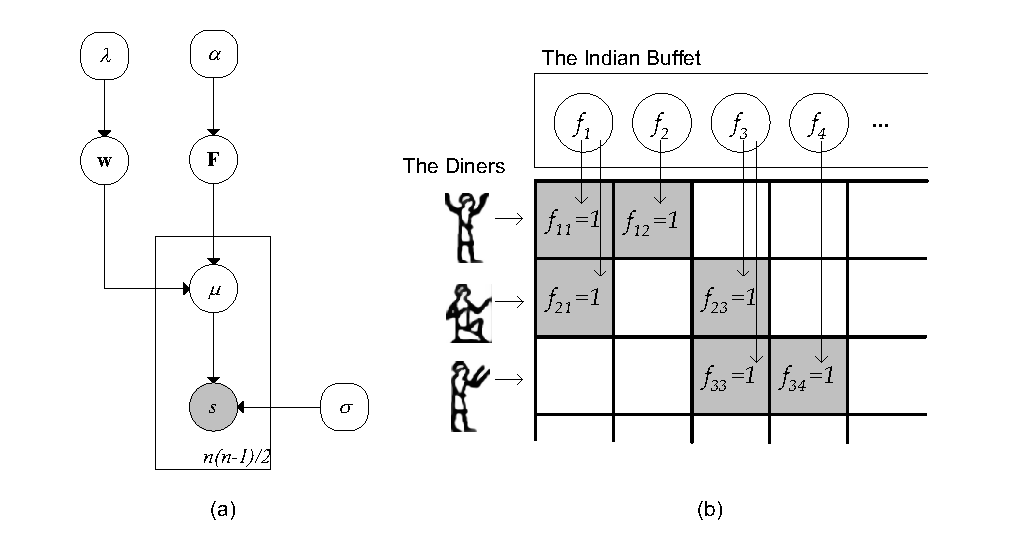
\epsfig{file=NECO-04-07-504-Figure5.eps, width=15cm}
\caption{\capspace Graphical model representation of the IBP-ADCLUS model. Panel (a) shows the hierarchical
structure of the ADCLUS model, and panel (b) illustrates the method by which a feature matrix is generated
using the Indian buffet process.}
\label{graphicalmodel}
\end{center}
\end{figure*}

Our approach to this problem employs the \emph{Indian buffet process} \cite<IBP;>{griffithsg05}, a simple stochastic process that generates samples from a distribution over sparse binary matrices with a fixed number of rows and an unbounded number of columns. This is particularly useful as a method for placing a prior over $\mathbf{F}$, since there is generally no good reason to assume an upper bound on the number of features that might be relevant to a particular similarity matrix. The IBP can be understood by imagining an Indian restaurant, in which there is a buffet table containing an infinite number of dishes. Each customer entering the restaurant samples a number of dishes from the buffet, with a preference for those dishes that other diners have tried. For the $k$th dish sampled by at least one of the first $i-1$ customers, the probability that the $i$th customer will also try that dish is
    \begin{equation}
    \label{ibp0}
    p(f_{ik}=1 | \mathbf{F}_{i-1}) = \frac{n_{k}}{i},
    \end{equation}
where ${\bf F}_{i-1}$ records the choices of the previous customers, and $n_k$ denotes the number of previous customers that have sampled that dish.  Being adventurous, the new customer may try some hitherto untasted meals from the infinite buffet on offer. The number of new dishes taken by customer $i$ follows a Poisson($\alpha/i$) distribution. Importantly, this sequential process generates {\it exchangeable} observations \cite<see>[for a precise treatment]{griffithsg05}. In other words, the probability of a binary feature matrix $\mathbf{F}$ does not depend on the order in which the customers appear (and is thus invariant under permutation of the rows). As a consequence, it is always possible to treat a particular observation as if it were the last one seen: much of the subsequent development in the paper relies on this property. As a consequence, we will often be interested in the special case of this equation corresponding to the $n$th customer, in which
    \begin{equation}
    \label{ibp}
    p(f_{nk}=1 | \mathbf{F}_{n-1}) = \frac{n_{k}}{n}.
    \end{equation}

If we assume that the ordering of the columns in the feature matrix is irrelevant to the model (which is true for additive clustering), then every binary feature matrix $\mathbf{F}$ is a member of a particular equivalence class $[\mathbf{F}]$, and it is at the level of these equivalence classes that we wish to specify our priors. Accordingly, we are interested in the distribution over equivalence classes from which the IBP generates samples \cite{griffithsg05}, which assigns probability to $[\mathbf{F}]$ as follows:
\begin{equation}
p([\mathbf{F}] \condon \alpha) = \frac{ \exp \left(- \alpha H_n \right) \alpha^m}{\prod_{h=1}^{2^n-1} m_h!} \prod_{k=1}^{m} \frac{(n-n_k)! (n_k-1)!}{n!},
\end{equation}
where $H_n$ denotes the $n$th harmonic number, $H_n = \sum_{j=1}^n 1/j$. In this expression, $h$ is an index variable that refers to one of the $2^n-1$ possible assignments of items to a particular feature, excluding the case where all elements are zero, and $m_h$ counts the number of features in $\mathbf{F}$ that have that particular pattern of assignments. To summarize, the nonparametric Bayesian additive clustering model may be written,
    \begin{equation}
    \begin{array}{rclcl}
    s_{ij} & \condon & \mathbf{F},\mathbf{w},\sigma &\sim &\mbox{Normal}(\mu_{ij},\sigma^2) \\
    w_k & \condon & \lambda_1, \lambda_2 & \sim & \mbox{Gamma}(\lambda_1, \lambda_2) \\
    \mathbf{F} & \condon & \alpha & \sim & \mbox{IBP}(\alpha).
    \end{array}
    \label{fullmodel}
    \end{equation}

With a fully specified statistical model in place, we are now in a position to discuss methods for performing the required inferences. Specifically, given the observed similarities $\mathbf{S}$, our goal is to infer the features $\mathbf{F}$ and saliencies $\mathbf{w}$ that underlie those data. To do so, we fix the hyperparameters $\alpha$, $\sigma$, $\lambda_1$ and $\lambda_2$, and then infer the posterior distribution over possible latent features. In the next two sections, we first discuss a numerical method for approximating this posterior distribution, and then move on to a discussion of the kinds of estimators that can be constructed from this distribution.

\presec \section{A Gibbs-Metropolis Sampling Scheme} \postsec

Having provided a complete specification of the model, we now turn to the question of how we can perform inference. As a Bayesian formulation of additive clustering, statistical inference in Equation~\ref{fullmodel} is based on the posterior distribution over feature matrices and saliency vectors, $p(\mathbf{F}, \mathbf{w} \condon \mathbf{S})$. Since the priors over $\mathbf{F}$ and $\mathbf{w}$ are independent, the application of Bayes' rule yields,
	\begin{equation}
	p(\mathbf{F}, \mathbf{w} \condon \mathbf{S}) = \frac{p(\mathbf{S} \condon \mathbf{F}, \mathbf{w})
	p(\mathbf{F}) p(\mathbf{w})}{p(\mathbf{S})}
	\end{equation}
where, for ease of exposition, we omit the dependence on the hyperparameters. Naturally, in any Bayesian model the ideal approach is to calculate posterior quantities using exact methods. Unfortunately, this is quite difficult in this case, particularly since the number of features is unbounded {\it a priori}. In view of this difficulty, a natural alternative is to use Markov chain Monte Carlo (MCMC) methods to repeatedly sample from the posterior distribution: estimates of posterior quantities can be made using these samples as proxies for the full distribution. Accordingly, we now describe a simple MCMC scheme for the Bayesian ADCLUS model, which uses a combination of Gibbs sampling \cite{gemang84} and more general Metropolis proposals \cite{metropolis53}.

The idea behind our procedure, as with all basic MCMC methods, is to start with randomly chosen values for $\mathbf{F}$ and $\mathbf{w}$, and update these values using a simple resampling procedure, discussed below. In our approach, at each step only a single $f_{ik}$ value or $w_k$ value is resampled; all other variables are held fixed at their pre-existing values. An iteration consists of a single sweep through all feature assignments and saliency weights. The logic behind the approach is that, irrespective of the starting point, a properly chosen sampling scheme will converge on samples from the ``target'' distribution, in this case the posterior distribution $p(\mathbf{F}, \mathbf{w} \condon \mathbf{S})$. A good introduction to the general approach, along with the conditions upon which MCMC convergence relies, is given by \citeA{gilks1995markov}. In the remainder of the section, we describe the sampling procedure that we used. The sampler is broken into three parts: (1) resampling a saliency $w_k$ for a feature $k$ that is currently non-empty (i.e., possessed by at least one item), (2) resampling a feature assignment $f_{ik}$, where $k$ again refers to a non-empty feature, and (3) resampling {\it all} the assignments and saliencies for the (infinite) set features that are currently empty. We discuss each part in turn.


{\it Saliency Weights (Non-Empty Features)}. When resampling the saliency of a non-empty feature, we use a Metropolis scheme with a Gaussian proposal distribution.\footnote{As with the Gamma prior over feature weights, the Gaussian proposal distribution for the sampler is not motivated by any strong theoretical reasons. It is simply a choice of convenience, and one that operates reasonably well in practice. In extensions currently under consideration, other choices for sampling schemes are being explored.} In other words, if the current state saliency is $w_k$, a candidate $w_k^*$ is first generated by drawing a sample from a Gaussian$(w_k, 0.05)$ distribution. The value of $w_k$ is then reassigned using the Metropolis update rule. If $\mathbf{w}_{-k}$ denotes the set of all saliencies except $w_k$, then this update rule can be written as
\begin{equation}
\begin{array}{cc}
w_k \leftarrow \left\{ \begin{array}{rl} w_k^* & \mbox{if } u<a \\ w_k & \mbox{otherwise} \end{array}\right. \!\!\! \mbox{, \hspace*{1mm} where }
a = \frac{p(\mathbf{S} \condon \mathbf{F}, \mathbf{w}_{-k}, w_k^*) p(w_k^*)}{p(\mathbf{S} \condon \mathbf{F}, \mathbf{w}_{-k}, w_k) p(w_k)}.
\end{array}
\end{equation}
In this expression, $u$ is a uniform random variate on the interval $[0,1)$. Note that, since the candidates are drawn from a Gaussian distribution, it is quite possible for the Metropolis sampler to propose replacement values $w_k^*$ that are less than zero. However, the Metropolis update rule will never accept one of these proposals, since $p(w_k^*)=0$ for all $w_k^* < 0$.

{\it Feature Assignments (Non-Empty Features)}. For features that are currently non-empty (i.e., $f_{ik}=1$ for at least one value of $i$), the feature assignments are updated using a standard Gibbs sampler: the value of $f_{ik}$ is drawn from the conditional posterior distribution over $f_{ik} \condon \mathbf{S},\mathbf{F}_{-ik},\mathbf{w}$. Since feature assignments are discrete, it is easy to find this conditional probability by noting that
    \begin{equation}
    p(f_{ik} | \mathbf{S},\mathbf{F}_{-ik},\mathbf{w}) \propto
    p(\mathbf{S} | \mathbf{F},\mathbf{w}) p(f_{ik} | \mathbf{F}_{-ik}),
    \end{equation}
where $\mathbf{F}_{-ik}$ denotes the set of all feature assignments except $f_{ik}$. The first term in this expression is just the likelihood function for the ADCLUS model, and is simple to calculate. Moreover, since feature assignments in the IBP are exchangeable \cite<see>[for details]{griffithsg05}, we can treat the $k$th assignment as if it were the last. Given this, Equation~\ref{ibp} indicates that $p(f_{ik} | \mathbf{F}_{-ik}) = n_{-ik}/n$, where $n_{-ik}$ counts the number of stimuli (besides the $i$th) that currently possess the $k$th feature. This analysis only applies to features for which $n_{-ik} > 0$. The remaining ``singleton'' features (i.e., those for which $f_{ik}=1$ for {\it exactly} one value of $i$) are identified when sweeping through all of the features associated with the $i$th object, and then deleted immediately before dealing with the features that are currently empty.

{\it Empty Features}. We now turn to how the sampler deals with the infinite set of currently-empty features. Since the IBP describes a prior over infinite feature matrices, the resampling procedure really does need to accommodate the remaining (infinite) set of features that are not currently represented among the manifest (i.e., non-empty) features. At a conceptual level it is helpful to note that if we were to redraw all these values simultaneously, some finite number of those currently-latent features would become manifest. In our MCMC procedure, we sample from the conditional posterior over feature assignments for the $i$th stimulus, holding all assignments fixed for the non-empty features, and also keeping the infinite set of (empty) feature assignments fixed for the other items. Now, in this case, if there were no data observed, this would be exactly equivalent to drawing the ``new'' features from the IBP. That is, we would introduce some number of ``singleton'' features possessed only by the $i$th object, where (due to exchangeability) this number is always drawn from a Poisson($\alpha/n$) distribution as noted previously. Fortunately, singleton features do not affect the probability of the data $\mathbf{S}$ in the additive clustering model, so the conditional posterior is exactly equivalent to the prior. In short, a very simple way to redraw for the infinite set of empty features is to sample Poisson($\alpha/n$) new singleton features for every stimulus. The weights for these singleton features are generated from the prior once those features are sampled.

When working with this algorithm, we typically run several chains. For each chain, we initialize the Gibbs-Metropolis sampler more or less arbitrarily. After a ``burn-in'' period is allowed for the sampler to converge to a sensible location  (i.e., for the state to represent a sample from the posterior), we make a ``draw'' by recording the state of the sampler, leaving a ``lag'' of several iterations between successive draws to reduce the autocorrelation between samples. When doing so, it is important to ensure that the Markov chains converge on the target distribution $p(\mathbf{F},\mathbf{w}\condon \mathbf{S})$. We did so by inspecting the time series plot formed by graphing the probability of successive samples. To illustrate this, one of the chains used in our simulations (see Section 5) is displayed in Figure~\ref{convergence}, with nine parallel chains used for comparison:  the time series plot shows no long-term trends, and that different chains are visually indistinguishable from one another.  Although elaborations and refinements are possible for both the sampler \cite{chen2000monte} and the convergence check \cite{cowles96}, we have found this approach to be reasonably effective for the moderate-sized problems considered in our applications.\footnote{One additional detail should be noted: sometimes the sampler proposes feature matrices that contain multiple copies of the `same' feature. While there are several possible ways to deal with this, for the sake of simplicity we report this as if only one copy of the feature were present, with a saliency equal to the sum of the copies.}


\begin{figure}
\begin{center}
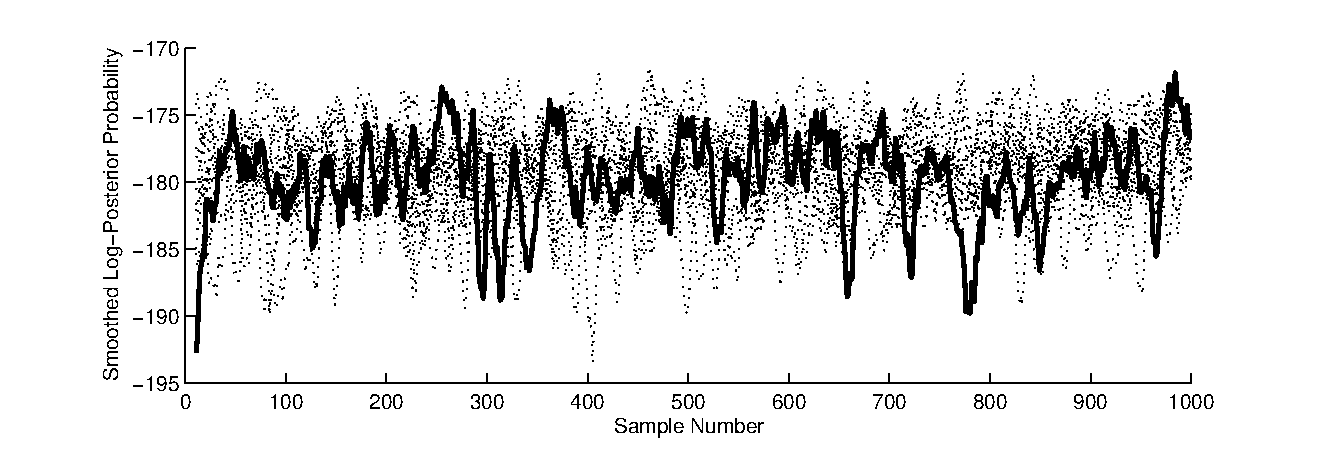
\epsfig{file=NECO-04-07-504-Figure6.eps, width=14cm}
\caption{\capspace Smoothed time series showing log-posterior probabilities for successive draws from the Gibbs-Metropolis sampler, for simulated similarity data with $n=16$. The bold line shows a single chain, while the dotted lines show the remaining nine chains. Note that, strictly speaking, since the normalizing contant for the posterior probability is unknown, the quantity being plotted differs from the actual log-probabilities by a constant.}
\label{convergence}
\end{center}
\end{figure}


\presec \section{Four Estimators for the ADCLUS Model} \postsec

One advantage to the IBP-ADCLUS approach is that it allows us to discuss a range of different estimators within a single framework. This is particularly useful since, in the absence of any explicit discussion of estimators, authors have adopted several different methods. The difficulty stems from the fact that there are several slightly different questions that one might wish to answer, and authors vary in the importance they attach to each. For instance,
\begin{enumerate}
\item How should features be assigned to stimuli? \vspace*{-9pt}
\item How much importance attaches to each feature? \vspace*{-9pt}
\item How many features should be included in the model? \vspace*{-9pt}
\item What predictions should be made about the similarities? \vspace*{-9pt}
\item What is the probability that a particular feature is represented?
\end{enumerate}
These are by no means the only questions that one could ask. For instance, question 5 is essentially about obtaining measures of uncertainty associated with the feature set $\mathbf{F}$. Accordingly, we could also ask for uncertainty estimates for the feature weights and the dimensionality of the model. However, we omit these questions for now, since all existing estimators can accommodate those in a natural fashion.

In this section we outline four different estimators that one might employ when using the additive clustering model, and show how each of the four relates to these different questions. As indicated, the key difference between the estimators is not the underlying model, nor the choice of utility function (though there are disagreements regarding these). The main issue here regards which parameters are ``nuisance parameters'' and which are ``parameters of interest''. In the Bayesian framework, if the parameter vector $\bm{\theta}=(\bm{\phi}, \bm{\lambda})$ can be partitioned into a set of interesting parameters $\bm{\phi}$ and a set of nuisance parameters $\bm{\lambda}$, it is typical to draw inferences about the interesting parameters using the marginal posterior:
\begin{equation}
p(\bm{\phi} \condon x) = \int p(\bm{\theta} \condon x) d\bm{\lambda} = \int p(\bm{\phi}, \bm{\lambda} \condon x) d\bm{\lambda}
\end{equation}
\cite<see>[p. 245]{bernardos00}. In the event that an estimate $\hat{\bm{\phi}}$ has already been obtained for the interesting parameters, it can be convenient to report estimates of the nuisance parameters conditional on the estimated values of the interesting parameters, using the conditional posterior distribution $p(\bm{\lambda} \condon \hat{\bm{\phi}}, x)$. This is often the case for the additive clustering model.


\subsection{Selecting the Posterior Mode}

The simplest approach to estimation in the additive clustering model is to report the posterior mode. This {\it maximum a posteriori} (MAP) estimator gives the single most likely set of parameter values, and is hence optimal under a 0-1 loss function. The MAP estimate is obtained by selecting the the feature matrix $\hat{\mathbf{F}}_1$ and saliency vector $\hat{\mathbf{w}}_1$ such that,
    \begin{equation}
    \hat{\mathbf{F}}_1, \hat{\mathbf{w}}_1 = \arg \max_{\mathbf{F},\mathbf{w}}
    p(\mathbf{F},\mathbf{w} \condon \mathbf{S}).
    \end{equation}
However, the MAP estimator is not generally used in additive clustering literature. The main reason for this is that the saturated model that contains a single two-stimulus feature for every cell in the similarity matrix can obtain perfect data fit by a judicious choice of weights. Accordingly, the only way to avoid this representation being chosen every time is to emphasize parsimony in either the prior or the loss function. In view of this obvious difficulty, the simple MAP estimator is almost never used. However, since many theoretically-motivated priors (including the IBP) allow the researcher to emphasize parsimony, it is possible to use this approach so long as one chooses the prior with care. Interestingly, this approach is paralleled in the frequentist literature: in order to produce parsimonious representations, some frequentist methods used in ADCLUS-like models apply penalty functions when obtaining a maximum likelihood feature model \cite{frankh06}.

When assessed in terms of the questions listed earlier, the simple MAP estimator gives priority to questions 1 and 2, since it is explicitly constructed to provide the best possible estimates (under 0-1 loss) for the features and weights. In contrast, it provides answers to the remaining questions only indirectly. The number of features $\hat{m}_1$ is implied by the feature matrix, and similarity predictions $\hat{\mathbf{S}}_1$ could be constructed using the reported features and saliencies. However, while some authors report measures of the uncertainty associated with the modal saliencies and number of features \cite<e.g.,>{frankh06}, it is not usual to report uncertainty measures for the specific features.


\subsection{Selecting the Most Likely Feature Set}


A rather different approach has been adopted by other authors \cite{lee02b,navarro03}, based on the typical application of the additive clustering model. The idea is that the saliency weights are of less psychological importance than the features to which they are applied, since saliencies often reflect context-specific levels of attention and are subject to frequent change. In contrast, the feature assignments themselves are usually treated as fixed properties of the stimulus representation \cite<e.g.,>{leen02}. Accordingly, the feature matrix $\mathbf{F}$ is taken to define a model with parameters $\mathbf{w}$. Under this view, the saliencies are treated as nuisance parameters, on the assumption that the psychologically important question is the identification of the feature matrix. Again based on a 0-1 loss function, the estimator $\hat{\mathbf{F}}_2$ for the feature matrix is then taken to be the marginal MAP feature set:
    \begin{equation}
    \hat{\mathbf{F}}_2 =\arg \max_{\mathbf{F}} p(\mathbf{F} \condon \mathbf{S})
    =  \arg \max_{\mathbf{F}} \left[  \int p(\mathbf{F},\mathbf{w} \condon \mathbf{S}) d\mathbf{w} \right].
    \label{mapfeature}
    \end{equation}
In general, the integral in Equation~\ref{mapfeature} is not tractable, so previous applications \cite<e.g.,>{lee02b,navarro03} have employed asymptotic approximations to $p(\mathbf{F} \condon \mathbf{S})$ for the sake of expediency, based on the Bayesian information criterion \cite{schwarz78}, Laplacian approximations \cite{debruijn58} or other related methods such as geometric complexity \cite{balasubramanian97} and minimum description length \cite{rissanen96}. Given the primacy of the feature matrix, it is then sensible to estimate the saliencies conditional on this estimate. The corresponding MAP estimator is thus,
\begin{equation}
\hat{\mathbf{w}}_2 = \arg \max_{\mathbf{w}} p(\mathbf{w} \condon \hat{\mathbf{F}}_2, \mathbf{S}).
\end{equation}
In this approach, the number of features $\hat{m}_2$ emerges as a consequence of the feature selection process, and similarity predictions $\hat{\mathbf{S}}_2$ would be made using the estimated features.
Thus, like the simpler MAP estimator outlined above, this approach considers questions 3 (dimensionality), 4 (prediction) and 5 (model uncertainty) to be of secondary importance. However, it differs in that it treats quesion 1 (feature selection) as being considerably more important than question 2 (feature weighting).


\subsection{Dimensionality Estimation and Conditional Posterior Modes}

The most common approach in the additive clustering literature is to divide the estimation problem into a model selection problem and a parameter estimation problem \cite{tenenbaum96,arabiec80,ruml02}. In this approach, the number of features $m$ is taken to define a particular model, with parameters corresponding to the $n \times m$ binary matrix $\mathbf{F}$ and the $m+1$ length vector $\mathbf{w}$. For the purposes of parameter estimation, neither $\mathbf{F}$ nor $\mathbf{w}$ are considered to be nuisance parameters, and so are estimated jointly. Again, assuming that we have some fixed value for $m$, we select the conditonally {\it maximum a posterior} (MAP) parameter values, given by
    \begin{equation}
    \hat{\mathbf{F}}_3, \hat{\mathbf{w}}_3 = \arg \max_{\mathbf{F},\mathbf{w}}
    p(\mathbf{F},\mathbf{w}     \condon \mathbf{S}, m)
    \label{constantmmap}
    \end{equation}
In practice, $m$ is rarely if ever known in advance. As a result, we need to solve a model selection problem in order to arrive at some estimate $\hat{m}_3$. When solving this problem, the psychologically-interesting variables $\mathbf{F}$ and $\mathbf{w}$ actually become the nuisance parameters. Accordingly, under 0-1 loss the (generally implicit) formulation of the model selection problem becomes,
    \begin{equation}
    \hat{m}_3 = \arg \max_m p(m \condon \mathbf{S}) = \arg \max_m \left[ \sum_{\mathbf{F} \in \mathcal{F}_m} \int
    p(\mathbf{F}, \mathbf{w} \condon \mathbf{S}) \ d\mathbf{w} \right].
    \label{posteriorm}
    \end{equation}
In this expression, $\mathcal{F}_m$ denotes the set of feature matrices containing $m$ unique features. The logic is that if we are to treat this as a model order selection problem, then the dimension $m$ defines a model that had parameters $\mathbf{F}$ and $\mathbf{w}$. Ideally, then, we would choose the most likely (or maximum utility) model $\hat{m}_3$ by integrating over the parameters of that model. Then, having estimated this model, we would report parameter values $\hat{\mathbf{F}}_3, \hat{\mathbf{w}}_3$ conditional on this model. In practice, given the difficulty of working with Equation~\ref{posteriorm}, it is typical to fix $m$ on the basis of intuition, or via some heuristic method. In terms of the four questions listed earlier, the model selection problem treats dimensionality (question 3) as the only question of interest, while the parameter estimation problem treats feature selection (question 1) and saliency (question 2) as equally important, given that the model selection problem has been solved. Again, the prediction (question 4) and feature uncertainty (question 5) are considered ancillary.


\subsection{Approximating the Posterior Predictive Similarity Matrix}

The three methods discussed above have all been applied to some extent in the existing literature. However, given that none are designed explicitly to address the questions of prediction and feature uncertainty, we now suggest a fourth possibility that complements the existing three. In this approach, we seek to uncover a small set of features that best approximates the posterior predictive similarity matrix. Letting $\hat{r}_k = p(\mathbf{f}_k \condon \mathbf{S})$ denote the posterior probability that feature $\mathbf{f}_k$ is manifest, we obtain
    \begin{equation}
    \hat{r}_k = p(\mathbf{f}_k \condon \mathbf{S}) = \sum_{\mathbf{F}: \mathbf{f}_k \in \mathbf{F}}
    p(\mathbf{F} \condon \mathbf{S}). \label{intpost}
    \end{equation}
This allows us to construct a vector $\hat{\mathbf{r}}=[\hat{r}_k]$ that contains these probabilities for all $2^n$ possible features. Although this vector discards the covariation between features across the posterior distribution, it is very useful, since the expected posterior similarities can be written as follows:
    \begin{eqnarray}
    \hat{s}_{ij} = E[{s_{ij}}^*|\mathbf{S}] &=& \sum_{\mathbf{f}_k} f_{ik} f_{jk} \hat{r}_k \hat{w}_k, \label{linear}
    \end{eqnarray}
where $\hat{w}_k = E\left[ w_k | \mathbf{f}_k, \mathbf{S} \right]$ denotes the expected saliency for feature $\mathbf{f}_k$ on those occasions when it is represented. Equation~\ref{linear} relies on the fact that features combine linearly in the ADCLUS model, and is straightforward to derive.

In practice, it is impossible to report all $2^n$ features, so although Equation~\ref{linear} provides the estimate  $\hat{\mathbf{S}}_4$ for the predicted similarities, one would typically report only those features that make the most substantial contributions to this estimate. While there are obviously several ways that we can formalize the notion of contribution, for the current purposes it will suffice to select those features for which $\hat{r}_k \hat{w}_k$ is largest. Similarly, there are several ways to determine the number of features to report, but for now we will simply ensure that the number of features reported for this method are in line with those suggested by the three existing methods.

Obviously, this approach treats prediction (question 4) as primary, but it is worth noting that since it involves the calculation of $\hat{r}_k$, the probability that feature $\mathbf{f}_k$ should be included in the representation, it gives some fairly explicit consideration to the question of feature uncertainty (question 5). This can be theoretically useful, since the concept of feature uncertainty is implicit in more general discussions of mental representation \cite{medino89} that ask whether or not a specific predicate is likely to be represented. However, unlike the other three estimators, it treats feature selection, feature saliency and dimensionality estimation (questions 1--3) as secondary.


\presec \section{Recovering Noisy Feature Matrices} \postsec
\begin{figure}
\begin{center}\hspace*{-2mm}
\begin{tabular}{cccc}
\raisebox{3.5cm}{\footnotesize \textsf{(a)}} \hspace*{-5mm} &
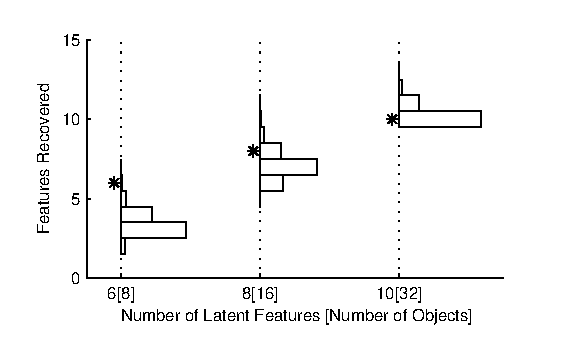
\epsfig{file=NECO-04-07-504-Figure7a.eps, width=7cm} &
\hspace*{-7mm} \raisebox{3.5cm}{\footnotesize \textsf{(b)}} & \hspace*{-2mm}
\raisebox{22mm}{\scriptsize
\begin{tabular}{|c|c|cccc|}
\hline
$n$ && $\hat{\mathbf{S}}_1$ & $\hat{\mathbf{S}}_2$ & $\hat{\mathbf{S}}_3$ & $\hat{\mathbf{S}}_4$ \\
\hline
&$\mathbf{S}_o$&    79&    81 &   79 &   84 \\
$8$&$\mathbf{S}_n$&    78&    81 &   78 &   84\\
& $\mathbf{S}_t$&   87&    88 &   87 &   92\\
\hline
& $\mathbf{S}_o$&   89 &   88 &   89 &   90\\
$16$& $\mathbf{S}_n$&   90 &   88 &   90  &  90\\
&$\mathbf{S}_t$&    96 &   95 &   96  &  97\\
\hline
&$\mathbf{S}_o$&    91  &  91  &  91 &   91\\
$32$& $\mathbf{S}_n$&   91  &  91  &  91  &  91\\
& $\mathbf{S}_t$&  100 &  100 &  100  & 100\\
\hline
\end{tabular}
\normalsize}
\end{tabular}
\caption{\capspace Posterior distributions (a) over the number of features $p(m\condon \mathbf{S}_o)$ in simulations containing $m_t=6$, $8$ and $10$ features respectively. Variance accounted for (b) by the four similarity estimators $\hat{\mathbf{S}}$, where the target is either the observed training data $\mathbf{S}_o$, a new test data set $\mathbf{S}_n$, or the true similarity matrix $\mathbf{S}_t$.}
\label{posteriorK}
\end{center}
\end{figure}
By using the IBP-ADCLUS framework, we can compare the performance of the four estimators in a reasonable fashion. Loosely following \citeA{ruml02}, we generated noisy similarity matrices with $n=8$, $16$ and $32$ stimuli, based on ``true''  feature matrices $\mathbf{F}_t$ in which $m_t=2\log_2(n)$, where each object possessed each feature with probability 0.5. Saliency weights $\mathbf{w}_t$ were generated uniformly from the interval $[1,3]$, but were subsequently rescaled to ensure that the ``true'' similarities $\mathbf{S}_t$ had variance 1. Two sets of Gaussian noise were injected into the similarities with fixed $\sigma=0.3$, ensuring that the noise accounted for approximately 9\% of the variance in the ``observed'' data matrix $\mathbf{S}_o$ and the ``new'' matrix $\mathbf{S}_n$. We fixed $\alpha=2$ for all simulations: since the number of manifest features in an IBP model follows a Poisson($\alpha H_n$) distribution \cite{griffithsg05}, the prior has a strong bias toward parsimony, since the prior expected number of features is approximately $5.4$, $6.8$ and $8.1$ (as compared to the true values of $6$, $8$ and $10$).

We approximated the posterior distribution $p(\mathbf{F},\mathbf{w}\condon \mathbf{S}_o)$, by drawing samples in the following manner. For a given similarity matrix, 10 Gibbs-Metropolis chains were run from different start points, and 1000 samples were drawn from each. The chains were burnt in for 1000 iterations, and a lag of 10 iterations was used  between successive samples. Visual inspection suggested that five chains in the $n=32$ condition did not converge: log-posteriors were low, differed substantially from one another, and had noticable positive slope. In this case, the estimators were constructed from the five remaining chains.

Figure~\ref{posteriorK}(a) shows the posterior distributions over the number of features $m$ for each of the three simulation conditions. There is a tendency to underestimate the number of features when provided with small similarity matrices, with the modal number being $3$, $7$ and $10$. However, since the posterior estimate of $m$ is below the prior estimate when $n=8$, it seems this effect is data-driven, as 79\% of the variance in the data matrix $\mathbf{S}_o$ can be accounted for using only three features.

Since each approach allows the construction of an estimated similarity matrix $\hat{\mathbf{S}}$, a natural comparison is to look at the proportion of variance this estimate accounts for in the observed data $\mathbf{S}_o$, the novel data set $\mathbf{S}_n$, and the true matrix $\mathbf{S}_t$. In view of the noise model used to construct these matrices, the ``ideal'' answer for these three should be around 91\%, 91\% and 100\% respectively. When $n=32$, this profile is observed for all four estimators, suggesting that in this case all four estimators have converged appropriately. For the smaller matrices, the joint MAP and conditional MAP estimators ($\hat{\mathbf{S}}_1$ and $\hat{\mathbf{S}}_3$) behave similarly. The MAP feature approach $\hat{\mathbf{S}}_2$ appears to perform slightly better, though the difference is very small. The expectation method $\hat{\mathbf{S}}_4$ provides the best estimate.

\begin{figure}[t]
\begin{center}\vspace*{-2mm}
\begin{tabular}{cccccc}
\raisebox{3.1cm}{\footnotesize \textsf{(a)}} &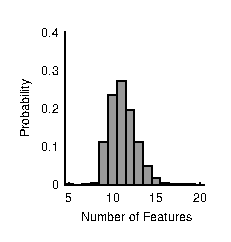
\epsfig{file=NECO-04-07-504-Figure8a.eps, width=3.2cm} &
\raisebox{3.1cm}{\footnotesize \textsf{(b)}} &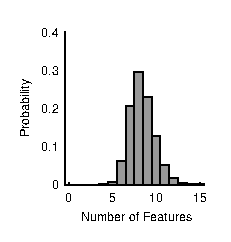
\epsfig{file=NECO-04-07-504-Figure8b.eps, width=3.2cm} &
\raisebox{3.1cm}{\footnotesize \textsf{(c)}} &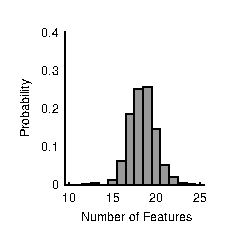
\epsfig{file=NECO-04-07-504-Figure8c.eps, width=3.2cm}
\end{tabular}
\end{center}
\caption{\capspace Posterior distributions over the number of features when the Bayesian ADCLUS model is applied to (a) the numbers data, (b) the countries data and (c) the letters data.}
\label{empdims}
\end{figure}


\presec \section{Modeling Empirical Similarities} \postsec

We now turn to the analysis of empirical data. To keep the presentation as brief as possible, we limit the discussion to the most novel IBP-ADCLUS estimators, namely the direct estimates of dimensionality provided through Equation~\ref{posteriorm}, and the features extracted via ``approximate expectation''.


\subsection{Featural representations of numbers.}

A standard data set used in evaluating additive clustering models measures the conceptual similarity of the numbers 0 through 9 \cite{shepardkc75}. This data set is often used as a benchmark due to the complex interrelationships between the numbers. Table~\ref{numreps}(a) shows an eight-feature representation of these data, taken from \citeA{tenenbaum96} who applied a maximum likelihood approach. This representation explains 90.9\% of the variance, with features corresponding to arithmetic concepts and to numerical magnitude. Fixing $\sigma=0.05$, and $\alpha=0.5$, we drew 10,000 lagged samples to construct estimates. Although the posterior probability is spread over a large number of feature matrices, 92.6\% of sampled matrices had between 9 and 13 features. The modal number of represented features was $\hat{m}_3$=11, with 27.2\% of the posterior mass. The posterior distribution over the number of features is shown in Figure~\ref{empdims}(a). Since none of the existing literature has used the ``approximate expectation'' approach to find highly probable features, it is useful to note the strong similarities between Table~\ref{numreps}(a) and Table~\ref{numreps}(b), which reports the ten highest-probability features across the entire posterior distribution. Applying this approach to obtain an estimate of the posterior predictive similarities $\hat{\mathbf{S}}_4$ revealed that this matrix accounts for 97.4\% of the variance in the data. Moreover, unlike the feature set reported by \citeA{tenenbaum96}, even and odd numbers both appear as distinct features.


\setlength{\tabcolsep}{2pt}
\begin{table}[t]
\caption{\capspace Two representations of the numbers data. (a) The
representation reported in \protect\cite{tenenbaum96}, extracted using
an EM algorithm with the number of features fixed at eight. (b)
The 10 most probable features extracted using the
Bayesian ADCLUS model. The first column gives the posterior probability
that a particular feature belongs in the representation. The second
column displays the average saliency of a feature in the event that it is
included. \vspace*{-5pt}}
\label{numreps} \begin{center}\footnotesize
  \begin{tabular}{cc}
    \raisebox{1.7cm}{\footnotesize \textsf{(a)} \ \ \ }
    \begin{tabular}{cccccccccccccc}\\
      \hline
      \multicolumn{10}{c}{\textsc{feature}}  & &\textsc{weight} \\
      \hline
      & & \texttt{2} & & \texttt{4} & & & & \texttt{8} & & & 0.444 \\[2pt]
      \texttt{0} & \texttt{1} & \texttt{2} & & & & & & &  & & 0.345 \\[2pt]
      & & & \texttt{3} & & & \texttt{6} & & & \texttt{9} & & 0.331 \\[2pt]
      & & & & & & \texttt{6} & \texttt{7} & \texttt{8} & \texttt{9} & & 0.291 \\[2pt]
      & & \texttt{2} & \texttt{3} & \texttt{4} & \texttt{5} & \texttt{6} & & & & & 0.255\\[2pt]
      & \texttt{1} & & \texttt{3} & & \texttt{5} & & \texttt{7} & & \texttt{9} & & 0.216 \\[2pt]
      & \texttt{1} & \texttt{2} & \texttt{3} & \texttt{4} & & & & & & & 0.214 \\[2pt]
      & & & & \texttt{4} & \texttt{5} & \texttt{6} & \texttt{7} & \texttt{8} & & & 0.172 \\[2pt]
      \multicolumn{10}{c}{additive constant} && 0.148 \\
      \hline
    \end{tabular} \hspace{5mm}
    &
    \raisebox{1.7cm}{\footnotesize \textsf{(b)} \ \ \ }
    \begin{tabular}{ccccccccccccccc}\\
      \hline
      \multicolumn{10}{c}{\textsc{feature}}  & &\textsc{prob.} & \textsc{weight}\\
      \hline
  &  &  & \texttt{3}  &  &  & \texttt{6}  &  &  & \texttt{9}  & & 0.79 & 0.326\\
  &  & \texttt{2}  &  & \texttt{4}  &  &  &  & \texttt{8}  &  & & 0.70 & 0.385\\
 \texttt{0}  & \texttt{1}  & \texttt{2}  &  &  &  &  &  &  &  & & 0.69 & 0.266\\
  &  & \texttt{2}  & \texttt{3}  & \texttt{4}  & \texttt{5}  & \texttt{6}  &  &  &  & & 0.59 & 0.240\\
  &  &  &  &  &  & \texttt{6}  & \texttt{7}  & \texttt{8}  & \texttt{9}  & & 0.57 & 0.262\\
 \texttt{0}  & \texttt{1}  & \texttt{2}  & \texttt{3}  & \texttt{4}  &  &  &  &  &  & & 0.42 & 0.173\\
  &  & \texttt{2}  &  & \texttt{4}  &  & \texttt{6}  &  & \texttt{8}  &  & & 0.41 & 0.387\\
  & \texttt{1}  &  & \texttt{3}  &  & \texttt{5}  &  & \texttt{7}  &  & \texttt{9}  & & 0.40 & 0.223\\
  &  &  &  & \texttt{4}  & \texttt{5}  & \texttt{6}  & \texttt{7}  & \texttt{8}  &  & & 0.34 & 0.181\\
  &  &  &  &  &  &  & \texttt{7}  & \texttt{8}  & \texttt{9}  & & 0.26 & 0.293\\
      \multicolumn{10}{c}{additive constant} && 1.00 & 0.075\\
      \hline
    \end{tabular}
\\ \\ \\
  \end{tabular}
  \normalsize \end{center} \end{table}


\subsection{Featural representations of countries}

A second application is to human forced-choice judgments of the similarities between 16 countries \cite{navarrol02}. In this task, participants were shown lists of four countries and asked to pick out the two countries most similar to each other. Applying the Bayesian model to these data with the empirically-estimated value of $\sigma=0.1$ reveals that only eight features appear in the representation more than 25\% of the time. Given this, it is not surprising that the posterior distribution over the number of features, shown in Figure~\ref{empdims}(b), indicates that the modal  number of features is eight. The eight most probable features are listed in Table~\ref{countries}. The ``approximate expectation'' method explains 85.4\% of the variance, as compared to the 78.1\% found by a MAP feature approach \cite{navarrol02}. The features are interpretable, corresponding to a range of geographical, historical, and economic regularities. Moreover, while the features recovered are very similar to those found by \citeA{navarrol02}, a comparison of the saliency weights reported in that paper (the ``NL-weight'' row in Table~\ref{countries}) to the saliencies and inclusion probabilities found here (the ``prob.'' and ``weight'' rows) reveals that there is considerable uncertainty associated with some features but not others, a fact that was not evident in the original paper. The first three features have $\hat{r}_k$ values that are very close to 1, whereas the other features may or may not form part of the underlying mental representation.


\setlength{\tabcolsep}{2pt}
\begin{table}[t]
\caption{\capspace Featural representation of the similarity between 16 countries. The table shows the eight highest-probability features extracted by the Bayesian ADCLUS model. Each column corresponds to a single feature, with the associated probabilities and saliencies shown below. The average weight associated with the additive constant is 0.035. The last line (NL-weight) lists the saliencies for the various features in the representation reported by \protect\citeA{navarrol02}.}
\label{countries} \begin{center}
\footnotesize
    \begin{tabular}{ccccccccc}\\
      \hline
      \multicolumn{9}{c}{\textsc{feature}} \\
      \hline
 &Italy & Vietnam & Germany & Zimbabwe & Zimbabwe & Iraq & Zimbabwe & Philippines \\
 &Germany & China & Russia & Nigeria & Nigeria & Libya & Nigeria & Indonesia \\
 &Spain & Japan &USA &  & Cuba &  & Iraq &   \\
 & & Philippines & China &  & Jamaica &  & Libya &  \\
 & & Indonesia & Japan &  & Iraq &  &  &  \\
 & &  &  &  & Libya &  &  &   \\
      \hline
\textsc{prob.} &
1.00   & 1.00 &   0.99&    0.62 &   0.52 &   0.36 &   0.33 &   0.25 \\
\textsc{weight} &    0.593 & 0.421&    0.267&    0.467&    0.209&
    0.373&    0.299&    0.311 \\
\\
\textsc{nl-weight} & 0.641 & 0.371 & 0.262 & 0.742 & - & 0.613 & - & 0.414 \\
\hline \\ \\
    \end{tabular}
\end{center}
\end{table}





\subsection{Featural Representations of Letters}

To provide a contrast with the last data set, in which there is considerably uncertainty associated with several of the features, we analyzed a somewhat larger data set, consisting of kindergarten children's assessment of the perceptual similarity of the 26 capital letters \cite{gibson63}. In this case, we used $\sigma = 0.05$, and the Bayesian model accounted for 89.2\% of the variance in the children's similarity judgments. The posterior distribution over the number of represented features is shown in Figure~\ref{empdims}(c). Table \ref{lettreps} shows the ten features that appeared in more than 90\% of samples from the posterior. The model recovers an extremely intuitive set of overlapping features. For example, it picks out the long strokes in \textsf{I}, \textsf{L}, and \textsf{T}, and the elliptical forms of \textsf{D}, \textsf{O}, and \textsf{Q}. Moreover, since the estimation method is sensitive to the full variation in the posterior distribution, we are able to say with a very high degree of certainty that all 10 features should be included as part of the inferred representation.


\begin{table}[t]
\caption{\capspace Featural representation of the perceptual similarity between 26 capital letters. The table shows the ten highest-probability features extracted by the Bayesian ADCLUS model. Each column corresponds to a single feature, with the associated probabilities and saliencies shown below. The average weight associated with the additive constant is 0.003.}
\label{lettreps} \begin{center}
\footnotesize
    \begin{tabular}{ccccccccccc}\\
      \hline
      \multicolumn{11}{c}{\textsc{feature}} \\
      \hline
 & \textsf{M} & \textsf{I} & \textsf{C} & \textsf{D} & \textsf{P} & \textsf{E} & \textsf{E} & \textsf{K} & \textsf{B} & \textsf{C} \\
 & \textsf{N} & \textsf{L} & \textsf{G} & \textsf{O} & \textsf{R} & \textsf{F} & \textsf{H} & \textsf{X} & \textsf{G} & \textsf{J} \\
 & \textsf{W} & \textsf{T} & & \textsf{Q} & & & & & \textsf{R} & \textsf{U} \\
      \hline
\textsc{prob.} & 1.00 & 0.99 & 0.99 & 0.99 & 0.99 & 0.99 & 0.99 & 0.99 & 0.98 & 0.92 \\
\textsc{weight} &  0.686 & 0.341 & 0.623 & 0.321 & 0.465 & 0.653 & 0.322 & 0.427 & 0.226 & 0.225 \\
\hline \\ \\
    \end{tabular}
\end{center}
\end{table}



\presec \section{Discussion} \postsec

Learning how similarity relations are represented is a difficult modeling problem. Additive clustering provides a framework for learning featural representations of stimulus similarity, but remains under-used due to the difficulties associated with the inference.  By adopting a Bayesian approach to additive clustering, we are able to obtain a richer characterization of the structure behind human similarity judgments. Moreover, by using nonparametric Bayesian techniques to place a prior distribution over infinite binary feature matrices via the Indian buffet process, we can allow the data to determine the number of features that the algorithm recovers. This is theoretically important as well as pragmatically useful. As noted by \citeA{medino89}, people are capable of recognizing that individual stimuli possess an arbitrarily large number of characteristics, but in any particular context will make judgments using only a finite, usually small number of properties that form part of our current mental representation. In other words, by moving to a Bayesian nonparametric form, we are able to bring the ADCLUS model closer to the kinds of assumptions that are made by psychological theories.

A number of avenues for extending this work present themselves. At a statistical level, placing hyperpriors over $\alpha$, $\sigma$ and $\lambda$ would seem to be a good idea, in order to infer their values from data. It would also be useful to switch to an extended version of the IBP, in which the implied prior over the number of features is decoupled from the implied prior over the number of objects that possess a particular feature. It may also be fruitful to consider stochastic featural similarity models that would allow one to infer whether two apparently-distinct features are simply noisy versions of one another. In order to scale the approach to larger domains, the MCMC algorithm could be augmented by using more advanced proposals \cite<e.g., split-merge steps;>{jainn04}. Psychologically, the ability to perform reliable inference in the ADCLUS model suggests that the model itself be extended to cover some of the more recent theoretical ideas in similarity. For instance, it would allow explicit testing of the ``size principle'' \cite{tenenbaumg01bbs}, which proposes on theoretical grounds that small features should be more salient on average. The underlying model itself could be extended from a pure common features model, to cover broader featural models \cite<e.g.,>{tversky77,navarrol04} and spatial-featural hybrids \cite<e.g.,>{navarrol03}. Further extensions could allow more complex, structured representations to be learned from data, in keeping with more recent theories for similarity and analogy \cite<e.g.,>{gen83,gol94c}. In the meantime, however, the adoption of a nonparametric Bayesian approach goes a long way towards making additive clustering a more reliable technique for recovering mental representations from human behavior.


\presec \section{Acknowledgments} \postsec

Correspondence concerning this article should be addressed to Daniel Navarro, School of Psychology, University of Adelaide, SA 5005, Australia, Tel.: +61 8 8303 5265, Fax.: +61 8 8303 3770, E-mail: daniel.navarro@adelaide.edu.au. Part of this work was presented at the 2006 {\it Neural Information Processing Systems} conference \cite<see>{navgriin}. DJN was supported by an Australian Research Fellowship (ARC grant DP-0773794). TLG was supported by a Junior Faculty Research Grant from the University of California, Berkeley and grant number BCS-0631518 from the National Science Foundation. We thank Nancy Briggs, Simon Dennis and Michael Lee for helpful comments. Matlab code implementing the procedures discussed in this paper are available on the first author's website.


%% Automatically generated bibliography:
\bibliographystyle{apacite}
\begin{thebibliography}{}
\setlength{\baselineskip}{24pt}

\bibitem[\protect\citeauthoryear{%
Aldous%
}{%
Aldous%
}{%
{\protect\APACyear{1985}}%
}]{%
aldous85}%
\APACinsertmetastar{%
aldous85}%
Aldous, D.%
%
\newblock{}\BBOP{}1985\BBCP{}.
\newblock{}\BBOQ{}Exchangeability and related topics.\BBCQ{}
\newblock{}\BIn{} \Bem{{\'E}cole d'{\'e}t{\'e} de probabilit{\'e}s de
  {S}aint-{F}lour, {XIII}---1983}\ (\BPGS\ 1--198).
\newblock{}Berlin: Springer.

\bibitem[\protect\citeauthoryear{%
Arabie%
\ \BBA{} Carroll%
}{%
Arabie%
\ \BBA{} Carroll%
}{%
{\protect\APACyear{1980}}%
}]{%
arabiec80}%
\APACinsertmetastar{%
arabiec80}%
Arabie, P.%
\BCBT{}\ \BBA{} Carroll, J.~D.%
%
\newblock{}\BBOP{}1980\BBCP{}.
\newblock{}\BBOQ{}{MAPCLUS}: A mathematical programming approach to fitting the
  {ADCLUS} model.\BBCQ{}
\newblock{}\Bem{Psychometrika}, \Bem{45}, 211-235.

\bibitem[\protect\citeauthoryear{%
Attneave%
}{%
Attneave%
}{%
{\protect\APACyear{1950}}%
}]{%
attneave50}%
\APACinsertmetastar{%
attneave50}%
Attneave, F.%
%
\newblock{}\BBOP{}1950\BBCP{}.
\newblock{}\BBOQ{}Dimensions of similarity.\BBCQ{}
\newblock{}\Bem{American Journal of Psychology}, \Bem{63}, 546-554.

\bibitem[\protect\citeauthoryear{%
Balasubramanian%
}{%
Balasubramanian%
}{%
{\protect\APACyear{1997}}%
}]{%
balasubramanian97}%
\APACinsertmetastar{%
balasubramanian97}%
Balasubramanian, V.%
%
\newblock{}\BBOP{}1997\BBCP{}.
\newblock{}\BBOQ{}Statistical inference, {O}ccam's razor, and statistical
  mechanics on the space of probability distributions.\BBCQ{}
\newblock{}\Bem{Neural computation}, \Bem{9}, 349-368.

\bibitem[\protect\citeauthoryear{%
Bernardo%
\ \BBA{} Smith%
}{%
Bernardo%
\ \BBA{} Smith%
}{%
{\protect\APACyear{2000}}%
}]{%
bernardos00}%
\APACinsertmetastar{%
bernardos00}%
Bernardo, J.~M.%
\BCBT{}\ \BBA{} Smith, A. F.~M.%
%
\newblock{}\BBOP{}2000\BBCP{}.
\newblock{}\Bem{Bayesian {T}heory (2nd ed)}.
\newblock{}New York: Wiley.

\bibitem[\protect\citeauthoryear{%
Blackwell%
\ \BBA{} MacQueen%
}{%
Blackwell%
\ \BBA{} MacQueen%
}{%
{\protect\APACyear{1973}}%
}]{%
blackwellm73}%
\APACinsertmetastar{%
blackwellm73}%
Blackwell, D.%
\BCBT{}\ \BBA{} MacQueen, J.%
%
\newblock{}\BBOP{}1973\BBCP{}.
\newblock{}\BBOQ{}Ferguson distributions via {P}olya urn schemes.\BBCQ{}
\newblock{}\Bem{The Annals of Statistics}, \Bem{1}, 353-355.

\bibitem[\protect\citeauthoryear{%
Browne%
}{%
Browne%
}{%
{\protect\APACyear{2001}}%
}]{%
browne01}%
\APACinsertmetastar{%
browne01}%
Browne, M.~W.%
%
\newblock{}\BBOP{}2001\BBCP{}.
\newblock{}\BBOQ{}An overview of analytic rotation in exploratory factor
  analysis.\BBCQ{}
\newblock{}\Bem{Multivariate Behavioral Research}, \Bem{36}, 111-150.

\bibitem[\protect\citeauthoryear{%
Buneman%
}{%
Buneman%
}{%
{\protect\APACyear{1971}}%
}]{%
buneman71}%
\APACinsertmetastar{%
buneman71}%
Buneman, P.%
%
\newblock{}\BBOP{}1971\BBCP{}.
\newblock{}\BBOQ{}The recovery of trees from measures of dissimilarity.\BBCQ{}
\newblock{}\BIn{} F.~R. Hodson, D.~G. Kendall\BCBL{}\ \BBA{} P.~Tautu\ (\BEDS),
  \Bem{Mathematics in the {A}rchaelogical and {H}istorical {S}ciences}\ (\BPG\
  387-395).
\newblock{}Edinburgh, UK: Edinburgh University Press.

\bibitem[\protect\citeauthoryear{%
Chen%
, Shao%
\BCBL{}\ \BBA{} Ibrahim%
}{%
Chen%
\ \protect\BOthers{.}}{%
{\protect\APACyear{2000}}%
}]{%
chen2000monte}%
\APACinsertmetastar{%
chen2000monte}%
Chen, M.%
, Shao, Q.%
\BCBL{}\ \BBA{} Ibrahim, J.~G.%
%
\newblock{}\BBOP{}2000\BBCP{}.
\newblock{}\Bem{Monte {Carlo} {Methods} in {Bayesian} {Computation}}.
\newblock{}New York, NY: Springer.

\bibitem[\protect\citeauthoryear{%
Cole%
\ \BBA{} Wishart%
}{%
Cole%
\ \BBA{} Wishart%
}{%
{\protect\APACyear{1970}}%
}]{%
colew70}%
\APACinsertmetastar{%
colew70}%
Cole, A.~J.%
\BCBT{}\ \BBA{} Wishart, D.%
%
\newblock{}\BBOP{}1970\BBCP{}.
\newblock{}\BBOQ{}An improved algorithm for the {J}ardine-{S}ibson method of
  generating overlapping clusters.\BBCQ{}
\newblock{}\Bem{The Computer Journal}, \Bem{13}, 156-163.

\bibitem[\protect\citeauthoryear{%
Corter%
\ \BBA{} Tversky%
}{%
Corter%
\ \BBA{} Tversky%
}{%
{\protect\APACyear{1986}}%
}]{%
cortert86}%
\APACinsertmetastar{%
cortert86}%
Corter, J.%
\BCBT{}\ \BBA{} Tversky, A.%
%
\newblock{}\BBOP{}1986\BBCP{}.
\newblock{}\BBOQ{}Extended similarity trees.\BBCQ{}
\newblock{}\Bem{Psychometrika}, \Bem{51}, 429-451.

\bibitem[\protect\citeauthoryear{%
Cowles%
\ \BBA{} Carlin%
}{%
Cowles%
\ \BBA{} Carlin%
}{%
{\protect\APACyear{1996}}%
}]{%
cowles96}%
\APACinsertmetastar{%
cowles96}%
Cowles, M.~K.%
\BCBT{}\ \BBA{} Carlin, B.~P.%
%
\newblock{}\BBOP{}1996\BBCP{}.
\newblock{}\BBOQ{}Markov chain {M}onte {C}arlo convergence diagnostics: {A}
  comparative review.\BBCQ{}
\newblock{}\Bem{Journal of the American Statistical Association}, \Bem{91},
  833-904.

\bibitem[\protect\citeauthoryear{%
Cunningham%
}{%
Cunningham%
}{%
{\protect\APACyear{1978}}%
}]{%
cunningham78}%
\APACinsertmetastar{%
cunningham78}%
Cunningham, J.~P.%
%
\newblock{}\BBOP{}1978\BBCP{}.
\newblock{}\BBOQ{}Free trees and bidirectional trees as representations of
  psychological distance.\BBCQ{}
\newblock{}\Bem{Journal of Mathematical Psychology}, \Bem{17}, 165-188.

\bibitem[\protect\citeauthoryear{%
D'Andrade%
}{%
D'Andrade%
}{%
{\protect\APACyear{1978}}%
}]{%
dandrade78}%
\APACinsertmetastar{%
dandrade78}%
D'Andrade, R.%
%
\newblock{}\BBOP{}1978\BBCP{}.
\newblock{}\BBOQ{}U-statistic hierarchical clustering.\BBCQ{}
\newblock{}\Bem{Psychometrika}, \Bem{4}, 58-67.

\bibitem[\protect\citeauthoryear{%
Dayhoff%
, Schwartz%
\BCBL{}\ \BBA{} Orcutt%
}{%
Dayhoff%
\ \protect\BOthers{.}}{%
{\protect\APACyear{1978}}%
}]{%
dayhoff78}%
\APACinsertmetastar{%
dayhoff78}%
Dayhoff, M.%
, Schwartz, R.%
\BCBL{}\ \BBA{} Orcutt, B.%
%
\newblock{}\BBOP{}1978\BBCP{}.
\newblock{}\BBOQ{}A model of evolutionary change in proteins.\BBCQ{}
\newblock{}\BIn{} M.~O. Dayhoff\ (\BED), \Bem{Atlas of {P}rotein {S}equence and
  {S}tructure 5(3)}\ (\BPG\ 345-352).
\newblock{}Washington: National Biomedical Research Foundation.

\bibitem[\protect\citeauthoryear{%
{de Bruijn}%
}{%
{de Bruijn}%
}{%
{\protect\APACyear{1958}}%
}]{%
debruijn58}%
\APACinsertmetastar{%
debruijn58}%
{de Bruijn}, N.~G.%
%
\newblock{}\BBOP{}1958\BBCP{}.
\newblock{}\Bem{Asymptotic Methods in Analysis}.
\newblock{}Amsterdam: North-Holland.

\bibitem[\protect\citeauthoryear{%
Dempster%
, Laird%
\BCBL{}\ \BBA{} Rubin%
}{%
Dempster%
\ \protect\BOthers{.}}{%
{\protect\APACyear{1977}}%
}]{%
dempsterlr77}%
\APACinsertmetastar{%
dempsterlr77}%
Dempster, A.~P.%
, Laird, N.~M.%
\BCBL{}\ \BBA{} Rubin, D.~B.%
%
\newblock{}\BBOP{}1977\BBCP{}.
\newblock{}\BBOQ{}Maximum likelihood from incomplete data via the {EM}
  algorithm.\BBCQ{}
\newblock{}\Bem{Journal of the Royal Statistical Society, B}, \Bem{39}.

\bibitem[\protect\citeauthoryear{%
Ekman%
}{%
Ekman%
}{%
{\protect\APACyear{1954}}%
}]{%
ekman54}%
\APACinsertmetastar{%
ekman54}%
Ekman, G.%
%
\newblock{}\BBOP{}1954\BBCP{}.
\newblock{}\BBOQ{}Dimensions of color vision.\BBCQ{}
\newblock{}\Bem{Journal of Psychology}, \Bem{38}, 467-474.

\bibitem[\protect\citeauthoryear{%
Ekman%
}{%
Ekman%
}{%
{\protect\APACyear{1963}}%
}]{%
ekman63}%
\APACinsertmetastar{%
ekman63}%
Ekman, G.%
%
\newblock{}\BBOP{}1963\BBCP{}.
\newblock{}\BBOQ{}A direct method for multidimensional ratio scaling.\BBCQ{}
\newblock{}\Bem{Psychometrika}, \Bem{28}, 33-41.

\bibitem[\protect\citeauthoryear{%
Escobar%
\ \BBA{} West%
}{%
Escobar%
\ \BBA{} West%
}{%
{\protect\APACyear{1995}}%
}]{%
escobarw95}%
\APACinsertmetastar{%
escobarw95}%
Escobar, M.~D.%
\BCBT{}\ \BBA{} West, M.%
%
\newblock{}\BBOP{}1995\BBCP{}.
\newblock{}\BBOQ{}Bayesian density estimation and inference using
  mixtures.\BBCQ{}
\newblock{}\Bem{Journal of the American Statistical Association}, \Bem{90},
  577-588.

\bibitem[\protect\citeauthoryear{%
Ferguson%
}{%
Ferguson%
}{%
{\protect\APACyear{1973}}%
}]{%
ferguson73}%
\APACinsertmetastar{%
ferguson73}%
Ferguson, T.~S.%
%
\newblock{}\BBOP{}1973\BBCP{}.
\newblock{}\BBOQ{}A {B}ayesian analysis of some nonparametric problems.\BBCQ{}
\newblock{}\Bem{The Annals of Statistics}, \Bem{1}, 209-230.

\bibitem[\protect\citeauthoryear{%
Ferguson%
}{%
Ferguson%
}{%
{\protect\APACyear{1974}}%
}]{%
ferguson74}%
\APACinsertmetastar{%
ferguson74}%
Ferguson, T.~S.%
%
\newblock{}\BBOP{}1974\BBCP{}.
\newblock{}\BBOQ{}Prior distributions on spaces of probability measures.\BBCQ{}
\newblock{}\Bem{Annals of Statistics}, \Bem{2}, 615-629.

\bibitem[\protect\citeauthoryear{%
Frank%
\ \BBA{} Heiser%
}{%
Frank%
\ \BBA{} Heiser%
}{%
{\protect\APACyear{in press}}%
}]{%
frankh06}%
\APACinsertmetastar{%
frankh06}%
Frank, L.~E.%
\BCBT{}\ \BBA{} Heiser, W.~J.%
%
\newblock{}\BBOP{}in press\BBCP{}.
\newblock{}\BBOQ{}Feature selection in {F}eature {N}etwork {M}odels: {F}inding
  predictive subsets of features with the {P}ositive {L}asso.\BBCQ{}
\newblock{}\Bem{British Journal of Mathematical and Statistical Psychology}.

\bibitem[\protect\citeauthoryear{%
Geman%
\ \BBA{} Geman%
}{%
Geman%
\ \BBA{} Geman%
}{%
{\protect\APACyear{1984}}%
}]{%
gemang84}%
\APACinsertmetastar{%
gemang84}%
Geman, S.%
\BCBT{}\ \BBA{} Geman, D.%
%
\newblock{}\BBOP{}1984\BBCP{}.
\newblock{}\BBOQ{}Stochastic relaxation, {G}ibbs distributions, and the
  {B}ayesian restoration of images.\BBCQ{}
\newblock{}\Bem{IEEE Transactions on Pattern Analysis and Machine
  Intelligence}, \Bem{6}, 721-741.

\bibitem[\protect\citeauthoryear{%
Gentner%
}{%
Gentner%
}{%
{\protect\APACyear{1983}}%
}]{%
gen83}%
\APACinsertmetastar{%
gen83}%
Gentner, D.%
%
\newblock{}\BBOP{}1983\BBCP{}.
\newblock{}\BBOQ{}Structure-mapping: A theoretical framework for
  analogy.\BBCQ{}
\newblock{}\Bem{Cognitive Science}, \Bem{7}, 155-170.

\bibitem[\protect\citeauthoryear{%
Gibson%
, Osser%
, Schiff%
\BCBL{}\ \BBA{} Smith%
}{%
Gibson%
\ \protect\BOthers{.}}{%
{\protect\APACyear{1963}}%
}]{%
gibson63}%
\APACinsertmetastar{%
gibson63}%
Gibson, E.~J.%
, Osser, H.%
, Schiff, W.%
\BCBL{}\ \BBA{} Smith, J.%
%
\newblock{}\BBOP{}1963\BBCP{}.
\newblock{}\Bem{An analysis of crictical features of letters, tested by a
  confusion matrix}\ (\BTR{}\ \BNUM\ Cooperative Research Project No. 639).
\newblock{}

\bibitem[\protect\citeauthoryear{%
Gilks%
, Richardson%
\BCBL{}\ \BBA{} Spiegelhalter%
}{%
Gilks%
\ \protect\BOthers{.}}{%
{\protect\APACyear{1995}}%
}]{%
gilks1995markov}%
\APACinsertmetastar{%
gilks1995markov}%
Gilks, W.~R.%
, Richardson, S.%
\BCBL{}\ \BBA{} Spiegelhalter, D.~J.%
%
\newblock{}\BBOP{}1995\BBCP{}.
\newblock{}\Bem{{M}arkov {C}hain {M}onte {C}arlo in {P}ractice}.
\newblock{}London, UK: Chapman and Hall.

\bibitem[\protect\citeauthoryear{%
Goldstone%
}{%
Goldstone%
}{%
{\protect\APACyear{1994}}%
}]{%
gol94c}%
\APACinsertmetastar{%
gol94c}%
Goldstone, R.~L.%
%
\newblock{}\BBOP{}1994\BBCP{}.
\newblock{}\BBOQ{}Similarity, interactive activation, and mapping.\BBCQ{}
\newblock{}\Bem{Journal of Experimental Psychology: Learning, Memory, and
  Cognition}, \Bem{20}, 3-28.

\bibitem[\protect\citeauthoryear{%
Goodman%
}{%
Goodman%
}{%
{\protect\APACyear{1972}}%
}]{%
goodman72}%
\APACinsertmetastar{%
goodman72}%
Goodman, N.%
%
\newblock{}\BBOP{}1972\BBCP{}.
\newblock{}\BBOQ{}Seven strictures on similarity.\BBCQ{}
\newblock{}\BIn{} N.~Goodman\ (\BED), \Bem{Problems and projects.}
\newblock{}New York: The Bobbs-Merrill Co.

\bibitem[\protect\citeauthoryear{%
Griffiths%
\ \BBA{} Ghahramani%
}{%
Griffiths%
\ \BBA{} Ghahramani%
}{%
{\protect\APACyear{2005}}%
}]{%
griffithsg05}%
\APACinsertmetastar{%
griffithsg05}%
Griffiths, T.~L.%
\BCBT{}\ \BBA{} Ghahramani, Z.%
%
\newblock{}\BBOP{}2005\BBCP{}.
\newblock{}\Bem{Infinite latent feature models and the {I}ndian buffet
  process}\ (\BTR{}\ \BNUM\ 2005-001).
\newblock{}Gatsby Computational Neuroscience Unit.

\bibitem[\protect\citeauthoryear{%
Hartigan%
\ \BBA{} Wong%
}{%
Hartigan%
\ \BBA{} Wong%
}{%
{\protect\APACyear{1979}}%
}]{%
hartiganw79}%
\APACinsertmetastar{%
hartiganw79}%
Hartigan, J.~A.%
\BCBT{}\ \BBA{} Wong, M.~A.%
%
\newblock{}\BBOP{}1979\BBCP{}.
\newblock{}\BBOQ{}Algorithm {AS} 136: A k-means clustering algorithm.\BBCQ{}
\newblock{}\Bem{Applied Statistics}, \Bem{28}, 100-108.

\bibitem[\protect\citeauthoryear{%
Henikoff%
\ \BBA{} Henikoff%
}{%
Henikoff%
\ \BBA{} Henikoff%
}{%
{\protect\APACyear{1992}}%
}]{%
henikoff92}%
\APACinsertmetastar{%
henikoff92}%
Henikoff, S.%
\BCBT{}\ \BBA{} Henikoff, J.%
%
\newblock{}\BBOP{}1992\BBCP{}.
\newblock{}\BBOQ{}Amino acid substitution matrices from protein blocks.\BBCQ{}
\newblock{}\Bem{Proceedings of the National Academy of Sciences USA}, \Bem{89},
  10915-10919.

\bibitem[\protect\citeauthoryear{%
Hotelling%
}{%
Hotelling%
}{%
{\protect\APACyear{1933}}%
}]{%
hotelling33}%
\APACinsertmetastar{%
hotelling33}%
Hotelling, H.%
%
\newblock{}\BBOP{}1933\BBCP{}.
\newblock{}\BBOQ{}Analysis of a complex of statistical variables into principal
  components.\BBCQ{}
\newblock{}\Bem{Journal of Educational Psychology}, \Bem{24}, 417-441, 498-520.

\bibitem[\protect\citeauthoryear{%
Hutchinson%
\ \BBA{} Mungale%
}{%
Hutchinson%
\ \BBA{} Mungale%
}{%
{\protect\APACyear{1997}}%
}]{%
hutchinsonm97}%
\APACinsertmetastar{%
hutchinsonm97}%
Hutchinson, J.~W.%
\BCBT{}\ \BBA{} Mungale, A.%
%
\newblock{}\BBOP{}1997\BBCP{}.
\newblock{}\BBOQ{}Pairwise partitioning: A nonmetric algorithm for identifying
  feature-based similarity structures.\BBCQ{}
\newblock{}\Bem{Psychometrika}, \Bem{62}, 85-117.

\bibitem[\protect\citeauthoryear{%
A.~K. Jain%
, Murty%
\BCBL{}\ \BBA{} Flynn%
}{%
A.~K. Jain%
\ \protect\BOthers{.}}{%
{\protect\APACyear{1999}}%
}]{%
jainmf99}%
\APACinsertmetastar{%
jainmf99}%
Jain, A.~K.%
, Murty, M.~N.%
\BCBL{}\ \BBA{} Flynn, P.~J.%
%
\newblock{}\BBOP{}1999\BBCP{}.
\newblock{}\BBOQ{}Data clustering: A review.\BBCQ{}
\newblock{}\Bem{ACM Computing Surveys}, \Bem{31}, 264-323.

\bibitem[\protect\citeauthoryear{%
S. Jain%
\ \BBA{} Neal%
}{%
S. Jain%
\ \BBA{} Neal%
}{%
{\protect\APACyear{2004}}%
}]{%
jainn04}%
\APACinsertmetastar{%
jainn04}%
Jain, S.%
\BCBT{}\ \BBA{} Neal, R.~M.%
%
\newblock{}\BBOP{}2004\BBCP{}.
\newblock{}\BBOQ{}A split-merge {M}arkov chain {M}onte {C}arlo procedure for
  the {D}irichlet {P}rocess mixture model.\BBCQ{}
\newblock{}\Bem{Journal of Computational and Graphical Statistics}, \Bem{13},
  158-182.

\bibitem[\protect\citeauthoryear{%
Jardine%
\ \BBA{} Sibson%
}{%
Jardine%
\ \BBA{} Sibson%
}{%
{\protect\APACyear{1968}}%
}]{%
jardines68}%
\APACinsertmetastar{%
jardines68}%
Jardine, N.%
\BCBT{}\ \BBA{} Sibson, R.%
%
\newblock{}\BBOP{}1968\BBCP{}.
\newblock{}\BBOQ{}The construction of hierarchic and non-hierarchic
  classifications.\BBCQ{}
\newblock{}\Bem{The Computer Journal}, \Bem{11}, 177-184.

\bibitem[\protect\citeauthoryear{%
Johnson%
}{%
Johnson%
}{%
{\protect\APACyear{1967}}%
}]{%
johnson67}%
\APACinsertmetastar{%
johnson67}%
Johnson, S.~C.%
%
\newblock{}\BBOP{}1967\BBCP{}.
\newblock{}\BBOQ{}Hierarchical clustering schemes.\BBCQ{}
\newblock{}\Bem{Psychometrika}, \Bem{32}, 241-254.

\bibitem[\protect\citeauthoryear{%
Komatsu%
}{%
Komatsu%
}{%
{\protect\APACyear{1992}}%
}]{%
komatsu92}%
\APACinsertmetastar{%
komatsu92}%
Komatsu, L.~K.%
%
\newblock{}\BBOP{}1992\BBCP{}.
\newblock{}\BBOQ{}Recent views of conceptual structure.\BBCQ{}
\newblock{}\Bem{Psychological Bulletin}, \Bem{112}(3), 500-526.

\bibitem[\protect\citeauthoryear{%
Kontkanen%
, Myllym\"{a}ki%
, Buntine%
, Rissanen%
\BCBL{}\ \BBA{} Tirri%
}{%
Kontkanen%
\ \protect\BOthers{.}}{%
{\protect\APACyear{2005}}%
}]{%
kontkanenmbrt05}%
\APACinsertmetastar{%
kontkanenmbrt05}%
Kontkanen, P.%
, Myllym\"{a}ki, P.%
, Buntine, W.%
, Rissanen, J.%
\BCBL{}\ \BBA{} Tirri, H.%
%
\newblock{}\BBOP{}2005\BBCP{}.
\newblock{}\BBOQ{}An {MDL} framework for data clustering.\BBCQ{}
\newblock{}\BIn{} \Bem{{A}dvances in {M}inimum {D}escription {L}ength: {T}heory and
  {A}pplications.}
\newblock{}Cambridge, MA: MIT Press.

\bibitem[\protect\citeauthoryear{%
Kraft%
}{%
Kraft%
}{%
{\protect\APACyear{1964}}%
}]{%
kraft64}%
\APACinsertmetastar{%
kraft64}%
Kraft, C.~H.%
%
\newblock{}\BBOP{}1964\BBCP{}.
\newblock{}\BBOQ{}A class of distribution function processes which have
  derivatives.\BBCQ{}
\newblock{}\Bem{Journal of Applied Probability}, \Bem{1}, 385-388.

\bibitem[\protect\citeauthoryear{%
Kruschke%
}{%
Kruschke%
}{%
{\protect\APACyear{1993}}%
}]{%
kruschke93}%
\APACinsertmetastar{%
kruschke93}%
Kruschke, J.~K.%
%
\newblock{}\BBOP{}1993\BBCP{}.
\newblock{}\BBOQ{}Human category learning: Implications for backpropagation
  models.\BBCQ{}
\newblock{}\Bem{Connection Science}, \Bem{5}, 3-36.

\bibitem[\protect\citeauthoryear{%
Kruskal%
}{%
Kruskal%
}{%
{\protect\APACyear{1964}}%
{\protect\APACexlab{{\protect\BCnt{1}}}}}]{%
kruskal64a}%
\APACinsertmetastar{%
kruskal64a}%
Kruskal, J.~B.%
%
\newblock{}\BBOP{}1964{\protect\BCnt{1}}\BBCP{}.
\newblock{}\BBOQ{}Multidimensional scaling by optimizing goodness of fit to a
  nonmetric hypothesis.\BBCQ{}
\newblock{}\Bem{Psychometrika}, \Bem{29}, 1-27.

\bibitem[\protect\citeauthoryear{%
Kruskal%
}{%
Kruskal%
}{%
{\protect\APACyear{1964}}%
{\protect\APACexlab{{\protect\BCnt{2}}}}}]{%
kruskal64b}%
\APACinsertmetastar{%
kruskal64b}%
Kruskal, J.~B.%
%
\newblock{}\BBOP{}1964{\protect\BCnt{2}}\BBCP{}.
\newblock{}\BBOQ{}Nonmetric multidimensional scaling: A numerical
  method.\BBCQ{}
\newblock{}\Bem{Psychometrika}, \Bem{29}, 115-129.

\bibitem[\protect\citeauthoryear{%
Landauer%
\ \BBA{} Dumais%
}{%
Landauer%
\ \BBA{} Dumais%
}{%
{\protect\APACyear{1997}}%
}]{%
landauerd97}%
\APACinsertmetastar{%
landauerd97}%
Landauer, T.~K.%
\BCBT{}\ \BBA{} Dumais, S.~T.%
%
\newblock{}\BBOP{}1997\BBCP{}.
\newblock{}\BBOQ{}A solution to {P}lato's problem: the {L}atent {S}emantic
  {A}nalysis theory of acquisition, induction, and representation of
  knowledge.\BBCQ{}
\newblock{}\Bem{Psychological Review}, \Bem{104}, 211-240.

\bibitem[\protect\citeauthoryear{%
Lawley%
\ \BBA{} Maxwell%
}{%
Lawley%
\ \BBA{} Maxwell%
}{%
{\protect\APACyear{1963}}%
}]{%
lawleym63}%
\APACinsertmetastar{%
lawleym63}%
Lawley, D.~N.%
\BCBT{}\ \BBA{} Maxwell, A.~E.%
%
\newblock{}\BBOP{}1963\BBCP{}.
\newblock{}\Bem{{F}actor {A}nalysis as a {S}tatistical {M}odel}.
\newblock{}London: Butterworths.

\bibitem[\protect\citeauthoryear{%
Lawson%
\ \BBA{} Hanson%
}{%
Lawson%
\ \BBA{} Hanson%
}{%
{\protect\APACyear{1974}}%
}]{%
lawhan74}%
\APACinsertmetastar{%
lawhan74}%
Lawson, C.~L.%
\BCBT{}\ \BBA{} Hanson, R.~J.%
%
\newblock{}\BBOP{}1974\BBCP{}.
\newblock{}\Bem{{S}olving {L}east {S}quares {P}roblems}.
\newblock{}Englewood Cliffs, NJ: Prentice-Hall.

\bibitem[\protect\citeauthoryear{%
Lee%
}{%
Lee%
}{%
{\protect\APACyear{1998}}%
}]{%
lee98}%
\APACinsertmetastar{%
lee98}%
Lee, M.~D.%
%
\newblock{}\BBOP{}1998\BBCP{}.
\newblock{}\BBOQ{}Neural feature abstraction from judgments of
  similarity.\BBCQ{}
\newblock{}\Bem{Neural Computation}, \Bem{10}(7), 1815-1830.

\bibitem[\protect\citeauthoryear{%
Lee%
}{%
Lee%
}{%
{\protect\APACyear{2001}}%
}]{%
lee01}%
\APACinsertmetastar{%
lee01}%
Lee, M.~D.%
%
\newblock{}\BBOP{}2001\BBCP{}.
\newblock{}\BBOQ{}Determining the dimensionality of multidimensional scaling
  models for cognitive modeling.\BBCQ{}
\newblock{}\Bem{Journal of Mathematical Psychology}, \Bem{45}, 149-166.

\bibitem[\protect\citeauthoryear{%
Lee%
}{%
Lee%
}{%
{\protect\APACyear{2002}}%
}]{%
lee02b}%
\APACinsertmetastar{%
lee02b}%
Lee, M.~D.%
%
\newblock{}\BBOP{}2002\BBCP{}.
\newblock{}\BBOQ{}Generating additive clustering models with limited stochastic
  complexity.\BBCQ{}
\newblock{}\Bem{Journal of Classification}, \Bem{19}, 69-85.

\bibitem[\protect\citeauthoryear{%
Lee%
\ \BBA{} Navarro%
}{%
Lee%
\ \BBA{} Navarro%
}{%
{\protect\APACyear{2002}}%
}]{%
leen02}%
\APACinsertmetastar{%
leen02}%
Lee, M.~D.%
\BCBT{}\ \BBA{} Navarro, D.~J.%
%
\newblock{}\BBOP{}2002\BBCP{}.
\newblock{}\BBOQ{}Extending the {ALCOVE} model of category learning to featural
  stimulus domains.\BBCQ{}
\newblock{}\Bem{Psychonomic Bulletin and Review}, \Bem{9}, 43-58.

\bibitem[\protect\citeauthoryear{%
Lee%
, Pincombe%
\BCBL{}\ \BBA{} Welsh%
}{%
Lee%
\ \protect\BOthers{.}}{%
{\protect\APACyear{2005}}%
}]{%
leepw05}%
\APACinsertmetastar{%
leepw05}%
Lee, M.~D.%
, Pincombe, B.~M.%
\BCBL{}\ \BBA{} Welsh, M.~B.%
%
\newblock{}\BBOP{}2005\BBCP{}.
\newblock{}\BBOQ{}An empirical evaluation of models of text document
  similarity.\BBCQ{}
\newblock{}\BIn{} \Bem{Proceedings of the 27th {A}nnual {C}onference of the
  {C}ognitive {S}cience {S}ociety}\ (\BPG\ 1254-1259).
\newblock{}Mahwah, NJ: Lawrence Erlbaum.

\bibitem[\protect\citeauthoryear{%
McAdams%
, Winsberg%
, Donnadieu%
, {de~Soete}%
\BCBL{}\ \BBA{} Krimphoff%
}{%
McAdams%
\ \protect\BOthers{.}}{%
{\protect\APACyear{1995}}%
}]{%
mcadams95}%
\APACinsertmetastar{%
mcadams95}%
McAdams, S.%
, Winsberg, S.%
, Donnadieu, S.%
, {de~Soete}, G.%
\BCBL{}\ \BBA{} Krimphoff, J.%
%
\newblock{}\BBOP{}1995\BBCP{}.
\newblock{}\BBOQ{}Perceptual scaling of synthesized musical timbres: Common
  dimensions, specificities, and latent subject classes.\BBCQ{}
\newblock{}\Bem{Psychological Research}, \Bem{58}, 177-192.

\bibitem[\protect\citeauthoryear{%
{McLachlan}%
\ \BBA{} {Basford}%
}{%
{McLachlan}%
\ \BBA{} {Basford}%
}{%
{\protect\APACyear{1988}}%
}]{%
mclachlanb88}%
\APACinsertmetastar{%
mclachlanb88}%
{McLachlan}, G.~J.%
\BCBT{}\ \BBA{} {Basford}, K.~E.%
%
\newblock{}\BBOP{}1988\BBCP{}.
\newblock{}\Bem{Mixture {M}odels. {I}nference and {A}pplications to {C}lustering}.
\newblock{}New York, NY: Dekker.

\bibitem[\protect\citeauthoryear{%
McQueen%
}{%
McQueen%
}{%
{\protect\APACyear{1967}}%
}]{%
mcqueen67}%
\APACinsertmetastar{%
mcqueen67}%
MacQueen, J.%
%
\newblock{}\BBOP{}1967\BBCP{}.
\newblock{}\BBOQ{}Some methods for classification and analysis of multivariate
  observations.\BBCQ{}
\newblock{}\BIn{} \Bem{Proceedings of the {F}ifth {B}erkeley {S}ymposium on
  {M}athematical {S}tatistics and {P}robability}\ (\BPG\ 281-297).
\newblock{}

\bibitem[\protect\citeauthoryear{%
Medin%
\ \BBA{} Ortony%
}{%
Medin%
\ \BBA{} Ortony%
}{%
{\protect\APACyear{1989}}%
}]{%
medino89}%
\APACinsertmetastar{%
medino89}%
Medin, D.~L.%
\BCBT{}\ \BBA{} Ortony, A.%
%
\newblock{}\BBOP{}1989\BBCP{}.
\newblock{}\BBOQ{}Psychological essentialism.\BBCQ{}
\newblock{}\BIn{} \Bem{Similarity and analogical reasoning.}
\newblock{}New York: Cambridge University Press.

\bibitem[\protect\citeauthoryear{%
Metropolis%
, Rosenbluth%
, Rosenbluth%
, Teller%
\BCBL{}\ \BBA{} Teller%
}{%
Metropolis%
\ \protect\BOthers{.}}{%
{\protect\APACyear{1953}}%
}]{%
metropolis53}%
\APACinsertmetastar{%
metropolis53}%
Metropolis, N.%
, Rosenbluth, A.~W.%
, Rosenbluth, M.~N.%
, Teller, A.~H.%
\BCBL{}\ \BBA{} Teller, E.%
%
\newblock{}\BBOP{}1953\BBCP{}.
\newblock{}\BBOQ{}Equations of state calculations by fast computing
  machines.\BBCQ{}
\newblock{}\Bem{Journal of Chemical Physics}, \Bem{21}, 1087-1092.

\bibitem[\protect\citeauthoryear{%
Minkowski%
}{%
Minkowski%
}{%
{\protect\APACyear{1891}}%
}]{%
minkowski1891}%
\APACinsertmetastar{%
minkowski1891}%
Minkowski, H.%
%
\newblock{}\BBOP{}1891\BBCP{}.
\newblock{}\BBOQ{}[on positive quadratic forms and on algorithms suggesting
  continued fractions].\BBCQ{}
\newblock{}\Bem{Journal f\"{u}r die reine und angewandte Mathematik},
  \Bem{107}, 278-297.

\bibitem[\protect\citeauthoryear{%
Mirkin%
}{%
Mirkin%
}{%
{\protect\APACyear{1987}}%
}]{%
mirkin87}%
\APACinsertmetastar{%
mirkin87}%
Mirkin, B.~G.%
%
\newblock{}\BBOP{}1987\BBCP{}.
\newblock{}\BBOQ{}Additive clustering and qualitative factor analysis methods
  for similarity matrices.\BBCQ{}
\newblock{}\Bem{Journal of Classification}, \Bem{4}, 7-31.

\bibitem[\protect\citeauthoryear{%
Myung%
, Balasubramanian%
\BCBL{}\ \BBA{} Pitt%
}{%
Myung%
\ \protect\BOthers{.}}{%
{\protect\APACyear{2000}}%
}]{%
myungbp00}%
\APACinsertmetastar{%
myungbp00}%
Myung, I.~J.%
, Balasubramanian, V.%
\BCBL{}\ \BBA{} Pitt, M.~A.%
%
\newblock{}\BBOP{}2000\BBCP{}.
\newblock{}\BBOQ{}Counting probability distributions: Differential geometry and
  model selection.\BBCQ{}
\newblock{}\Bem{Proceedings of the National Academy of Sciences}, \Bem{97},
  11170-11175.

\bibitem[\protect\citeauthoryear{%
Navarro%
}{%
Navarro%
}{%
{\protect\APACyear{2003}}%
}]{%
navarro03}%
\APACinsertmetastar{%
navarro03}%
Navarro, D.~J.%
%
\newblock{}\BBOP{}2003\BBCP{}.
\newblock{}\Bem{Representing stimulus similarity}.
\newblock{}Ph.D. Thesis, University of Adelaide.

\bibitem[\protect\citeauthoryear{%
Navarro%
\ \BBA{} Griffiths%
}{%
Navarro%
\ \BBA{} Griffiths%
}{%
{\protect\APACyear{2007}}%
}]{%
navgriin}%
\APACinsertmetastar{%
navgriin}%
Navarro, D.~J.%
\BCBT{}\ \BBA{} Griffiths, T.~L.%
%
\newblock{}\BBOP{}2007\BBCP{}.
\newblock{}\BBOQ{}A nonparametric Bayesian method for inferring features from
  similarity judgments.\BBCQ{}
\newblock{}\BIn{} \Bem{Advances in Neural Information Processing Systems, 19} \ (\BPG\ 1033-1040).
\newblock{}Cambridge, MA: MIT Press.

\bibitem[\protect\citeauthoryear{%
Navarro%
, Griffiths%
, Steyvers%
\BCBL{}\ \BBA{} Lee%
}{%
Navarro%
\ \protect\BOthers{.}}{%
{\protect\APACyear{2006}}%
}]{%
navarrogsl06}%
\APACinsertmetastar{%
navarrogsl06}%
Navarro, D.~J.%
, Griffiths, T.~L.%
, Steyvers, M.%
\BCBL{}\ \BBA{} Lee, M.~D.%
%
\newblock{}\BBOP{}2006\BBCP{}.
\newblock{}\BBOQ{}Modeling individual differences using {D}irichlet
  processes.\BBCQ{}
\newblock{}\Bem{Journal of Mathematical Psychology}, \Bem{50}, 101-122.

\bibitem[\protect\citeauthoryear{%
Navarro%
\ \BBA{} Lee%
}{%
Navarro%
\ \BBA{} Lee%
}{%
{\protect\APACyear{2002}}%
}]{%
navarrol02}%
\APACinsertmetastar{%
navarrol02}%
Navarro, D.~J.%
\BCBT{}\ \BBA{} Lee, M.~D.%
%
\newblock{}\BBOP{}2002\BBCP{}.
\newblock{}\BBOQ{}Commonalities and distinctions in featural stimulus
  representations.\BBCQ{}
\newblock{}\BIn{} \Bem{Proceedings of the 24th {A}nnual {C}onference of the
  {C}ognitive {S}cience {S}ociety}\ (\BPG\ 685-690).
\newblock{}Mahwah, NJ: Lawrence Erlbaum.

\bibitem[\protect\citeauthoryear{%
Navarro%
\ \BBA{} Lee%
}{%
Navarro%
\ \BBA{} Lee%
}{%
{\protect\APACyear{2003}}%
}]{%
navarrol03}%
\APACinsertmetastar{%
navarrol03}%
Navarro, D.~J.%
\BCBT{}\ \BBA{} Lee, M.~D.%
%
\newblock{}\BBOP{}2003\BBCP{}.
\newblock{}\BBOQ{}Combining dimensions and features in similarity-based
  representations.\BBCQ{}
\newblock{}\BIn{} \Bem{Advances in {N}eural {I}nformation {P}rocessing
  {S}ystems 15.} \ (\BPG\ 67-74)
\newblock{}Cambridge, MA: MIT Press.

\bibitem[\protect\citeauthoryear{%
Navarro%
\ \BBA{} Lee%
}{%
Navarro%
\ \BBA{} Lee%
}{%
{\protect\APACyear{2004}}%
}]{%
navarrol04}%
\APACinsertmetastar{%
navarrol04}%
Navarro, D.~J.%
\BCBT{}\ \BBA{} Lee, M.~D.%
%
\newblock{}\BBOP{}2004\BBCP{}.
\newblock{}\BBOQ{}Common and distinctive features in stimulus representation: A
  modified version of the contrast model.\BBCQ{}
\newblock{}\Bem{Psychonomic Bulletin and Review}, \Bem{11}, 961-974.

\bibitem[\protect\citeauthoryear{%
Neal%
}{%
Neal%
}{%
{\protect\APACyear{2003}}%
}]{%
neal03}%
\APACinsertmetastar{%
neal03}%
Neal, R.~M.%
%
\newblock{}\BBOP{}2003\BBCP{}.
\newblock{}\BBOQ{}Density modeling and clustering using {D}irichlet diffusion
  trees.\BBCQ{}
\newblock{}\Bem{Bayesian Statistics}, \Bem{7}, 619-629.

\bibitem[\protect\citeauthoryear{%
Pearson%
}{%
Pearson%
}{%
{\protect\APACyear{1901}}%
}]{%
pearson1901}%
\APACinsertmetastar{%
pearson1901}%
Pearson, K.%
%
\newblock{}\BBOP{}1901\BBCP{}.
\newblock{}\BBOQ{}On lines and planes of closest fit to a system of points in
  space.\BBCQ{}
\newblock{}\Bem{Philosophical Magazine}, \Bem{2}, 559-572.

\bibitem[\protect\citeauthoryear{%
Pitman%
}{%
Pitman%
}{%
{\protect\APACyear{1996}}%
}]{%
pitman96}%
\APACinsertmetastar{%
pitman96}%
Pitman, J.%
%
\newblock{}\BBOP{}1996\BBCP{}.
\newblock{}\BBOQ{}Some developments of the {B}lackwell-{M}ac{Q}ueen urn
  scheme.\BBCQ{}
\newblock{}\BIn{} T.~F. et al\ (\BED), \Bem{Statistics, {P}robability and {G}ame
  {T}heory: Papers in {H}onor of {D}avid {B}lackwell}\ (\BPG\ 245-267).
\newblock{}Hayward, CA: Institute of Mathematical Studies.

\bibitem[\protect\citeauthoryear{%
Ramsay%
}{%
Ramsay%
}{%
{\protect\APACyear{1982}}%
}]{%
ramsay82}%
\APACinsertmetastar{%
ramsay82}%
Ramsay, J.~O.%
%
\newblock{}\BBOP{}1982\BBCP{}.
\newblock{}\BBOQ{}Some statistical approaches to multidimensional scaling
  data.\BBCQ{}
\newblock{}\Bem{Journal of the Royal Statistical Society. Series A (General)},
  \Bem{145}, 285-312.

\bibitem[\protect\citeauthoryear{%
Rasmussen%
}{%
Rasmussen%
}{%
{\protect\APACyear{2000}}%
}]{%
rasmussen00}%
\APACinsertmetastar{%
rasmussen00}%
Rasmussen, C.%
%
\newblock{}\BBOP{}2000\BBCP{}.
\newblock{}\BBOQ{}The infinite {G}aussian mixture model.\BBCQ{}
\newblock{}\BIn{} \Bem{Advances in {N}eural {I}nformation {P}rocessing
  {S}ystems 12.}
\newblock{}Cambridge, MA: MIT Press.

\bibitem[\protect\citeauthoryear{%
Rissanen%
}{%
Rissanen%
}{%
{\protect\APACyear{1996}}%
}]{%
rissanen96}%
\APACinsertmetastar{%
rissanen96}%
Rissanen, J.%
%
\newblock{}\BBOP{}1996\BBCP{}.
\newblock{}\BBOQ{}Fisher information and stochastic complexity.\BBCQ{}
\newblock{}\Bem{IEEE Transactions on Information Theory}, \Bem{42}(1), 40-47.

\bibitem[\protect\citeauthoryear{%
Rosenberg%
\ \BBA{} Kim%
}{%
Rosenberg%
\ \BBA{} Kim%
}{%
{\protect\APACyear{1975}}%
}]{%
rosenbergk75}%
\APACinsertmetastar{%
rosenbergk75}%
Rosenberg, S.%
\BCBT{}\ \BBA{} Kim, M.~P.%
%
\newblock{}\BBOP{}1975\BBCP{}.
\newblock{}\BBOQ{}The method of sorting as a data-generating procedure in
  multivariate research.\BBCQ{}
\newblock{}\Bem{Multivariate Behavioral Research}, \Bem{10}, 489-502.

\bibitem[\protect\citeauthoryear{%
Ruml%
}{%
Ruml%
}{%
{\protect\APACyear{2001}}%
}]{%
ruml02}%
\APACinsertmetastar{%
ruml02}%
Ruml, W.%
%
\newblock{}\BBOP{}2001\BBCP{}.
\newblock{}\BBOQ{}Constructing distributed representations using additive
  clustering.\BBCQ{}
\newblock{}\BIn{} \Bem{Advances in {N}eural {I}nformation {P}rocessing
  {S}ystems 14.}
\newblock{}Cambridge, MA: MIT Press.

\bibitem[\protect\citeauthoryear{%
Sattath%
\ \BBA{} Tversky%
}{%
Sattath%
\ \BBA{} Tversky%
}{%
{\protect\APACyear{1977}}%
}]{%
sattatht77}%
\APACinsertmetastar{%
sattatht77}%
Sattath, S.%
\BCBT{}\ \BBA{} Tversky, A.%
%
\newblock{}\BBOP{}1977\BBCP{}.
\newblock{}\BBOQ{}Additive similarity trees.\BBCQ{}
\newblock{}\Bem{Psychometrika}, \Bem{42}, 319-345.

\bibitem[\protect\citeauthoryear{%
Schwarz%
}{%
Schwarz%
}{%
{\protect\APACyear{1978}}%
}]{%
schwarz78}%
\APACinsertmetastar{%
schwarz78}%
Schwarz, G.%
%
\newblock{}\BBOP{}1978\BBCP{}.
\newblock{}\BBOQ{}Estimating the dimension of a model.\BBCQ{}
\newblock{}\Bem{The Annals of Statistics}, \Bem{6}(2), 461-464.

\bibitem[\protect\citeauthoryear{%
Sethuraman%
}{%
Sethuraman%
}{%
{\protect\APACyear{1994}}%
}]{%
sethuraman94}%
\APACinsertmetastar{%
sethuraman94}%
Sethuraman, J.%
%
\newblock{}\BBOP{}1994\BBCP{}.
\newblock{}\BBOQ{}A constructive definition of {D}irichlet priors.\BBCQ{}
\newblock{}\Bem{Statistica Sinica}, \Bem{4}, 639-650.

\bibitem[\protect\citeauthoryear{%
Shepard%
}{%
Shepard%
}{%
{\protect\APACyear{1962}}%
}]{%
shepard62}%
\APACinsertmetastar{%
shepard62}%
Shepard, R.~N.%
%
\newblock{}\BBOP{}1962\BBCP{}.
\newblock{}\BBOQ{}The analysis of proximities: Multidimensional scaling with
  and unknown distance function. {I} and {II}.\BBCQ{}
\newblock{}\Bem{Psychometrika}, \Bem{27}, 125-140, 219-246.

\bibitem[\protect\citeauthoryear{%
Shepard%
}{%
Shepard%
}{%
{\protect\APACyear{1972}}%
}]{%
shepard72}%
\APACinsertmetastar{%
shepard72}%
Shepard, R.~N.%
%
\newblock{}\BBOP{}1972\BBCP{}.
\newblock{}\BBOQ{}Psychological representation of speech sounds.\BBCQ{}
\newblock{}\BIn{} E.~E. David\ \BBA{} P.~B. Denes\ (\BEDS), \Bem{Human
  {C}ommunication: A {U}nified {V}iew}\ (\BPG\ 67-113).
\newblock{}New York, NY: McGraw-Hill.

\bibitem[\protect\citeauthoryear{%
Shepard%
\ \BBA{} Arabie%
}{%
Shepard%
\ \BBA{} Arabie%
}{%
{\protect\APACyear{1979}}%
}]{%
sheparda79}%
\APACinsertmetastar{%
sheparda79}%
Shepard, R.~N.%
\BCBT{}\ \BBA{} Arabie, P.%
%
\newblock{}\BBOP{}1979\BBCP{}.
\newblock{}\BBOQ{}Additive clustering: Representation of similarities as
  combinations of discrete overlapping properties.\BBCQ{}
\newblock{}\Bem{Psychological Review}, \Bem{86}, 87-123.

\bibitem[\protect\citeauthoryear{%
Shepard%
, Kilpatric%
\BCBL{}\ \BBA{} Cunningham%
}{%
Shepard%
\ \protect\BOthers{.}}{%
{\protect\APACyear{1975}}%
}]{%
shepardkc75}%
\APACinsertmetastar{%
shepardkc75}%
Shepard, R.~N.%
, Kilpatric, D.~W.%
\BCBL{}\ \BBA{} Cunningham, J.~P.%
%
\newblock{}\BBOP{}1975\BBCP{}.
\newblock{}\BBOQ{}The internal representation of numbers.\BBCQ{}
\newblock{}\Bem{Cognitive Psychology}, \Bem{7}, 82-138.

\bibitem[\protect\citeauthoryear{%
Sneath%
}{%
Sneath%
}{%
{\protect\APACyear{1957}}%
}]{%
sneath57}%
\APACinsertmetastar{%
sneath57}%
Sneath, P. H.~A.%
%
\newblock{}\BBOP{}1957\BBCP{}.
\newblock{}\BBOQ{}The application of computers to taxonomy.\BBCQ{}
\newblock{}\Bem{The Journal of General Microbiology}, \Bem{17}, 201-206.

\bibitem[\protect\citeauthoryear{%
Sokal%
}{%
Sokal%
}{%
{\protect\APACyear{1974}}%
}]{%
sokal74}%
\APACinsertmetastar{%
sokal74}%
Sokal, R.~R.%
%
\newblock{}\BBOP{}1974\BBCP{}.
\newblock{}\BBOQ{}Classification: Purposes, principles, progress,
  prospects.\BBCQ{}
\newblock{}\Bem{Science}, \Bem{185}, 1115-1123.

\bibitem[\protect\citeauthoryear{%
Sokal%
\ \BBA{} Sneath%
}{%
Sokal%
\ \BBA{} Sneath%
}{%
{\protect\APACyear{1963}}%
}]{%
sokals63}%
\APACinsertmetastar{%
sokals63}%
Sokal, R.~R.%
\BCBT{}\ \BBA{} Sneath, P. H.~A.%
%
\newblock{}\BBOP{}1963\BBCP{}.
\newblock{}\Bem{Principles of {N}umerical {T}axonomy}.
\newblock{}San Francisco: Freeman.

\bibitem[\protect\citeauthoryear{%
Spearman%
}{%
Spearman%
}{%
{\protect\APACyear{1904}}%
}]{%
spearman04}%
\APACinsertmetastar{%
spearman04}%
Spearman, C.%
%
\newblock{}\BBOP{}1904\BBCP{}.
\newblock{}\BBOQ{}General intelligence, objectively determined and
  measured.\BBCQ{}
\newblock{}\Bem{American Journal of Psychology}, \Bem{15}, 201-293.

\bibitem[\protect\citeauthoryear{%
Spearman%
}{%
Spearman%
}{%
{\protect\APACyear{1927}}%
}]{%
spearman27}%
\APACinsertmetastar{%
spearman27}%
Spearman, C.%
%
\newblock{}\BBOP{}1927\BBCP{}.
\newblock{}\Bem{The {A}bilities of {M}an}.
\newblock{}New York: Macmillan.

\bibitem[\protect\citeauthoryear{%
Stevens%
}{%
Stevens%
}{%
{\protect\APACyear{1946}}%
}]{%
stevens46}%
\APACinsertmetastar{%
stevens46}%
Stevens, S.~S.%
%
\newblock{}\BBOP{}1946\BBCP{}.
\newblock{}\BBOQ{}On the theory of scales of measurement.\BBCQ{}
\newblock{}\Bem{Science}, \Bem{103}, 677-680.

\bibitem[\protect\citeauthoryear{%
Stevens%
}{%
Stevens%
}{%
{\protect\APACyear{1951}}%
}]{%
stevens51}%
\APACinsertmetastar{%
stevens51}%
Stevens, S.~S.%
%
\newblock{}\BBOP{}1951\BBCP{}.
\newblock{}\BBOQ{}Mathematics, measurement, and psychophysics.\BBCQ{}
\newblock{}\BIn{} \Bem{Handbook of {E}xperimental {P}sychology.}
\newblock{}New York: Wiley.

\bibitem[\protect\citeauthoryear{%
Tenenbaum%
}{%
Tenenbaum%
}{%
{\protect\APACyear{1996}}%
}]{%
tenenbaum96}%
\APACinsertmetastar{%
tenenbaum96}%
Tenenbaum, J.~B.%
%
\newblock{}\BBOP{}1996\BBCP{}.
\newblock{}\BBOQ{}Learning the structure of similarity.\BBCQ{}
\newblock{}\BIn{} D.~S. Touretzky, M.~C. Mozer\BCBL{}\ \BBA{} M.~E. Hasselmo\
  (\BEDS), \Bem{Advances in {N}eural {I}nformation {P}rocessing {S}ystems}\
  (\BVOL~8, \BPG\ 3-9).
\newblock{}Cambridge, MA: MIT Press.

\bibitem[\protect\citeauthoryear{%
Tenenbaum%
\ \BBA{} Griffiths%
}{%
Tenenbaum%
\ \BBA{} Griffiths%
}{%
{\protect\APACyear{2001}}%
}]{%
tenenbaumg01bbs}%
\APACinsertmetastar{%
tenenbaumg01bbs}%
Tenenbaum, J.~B.%
\BCBT{}\ \BBA{} Griffiths, T.~L.%
%
\newblock{}\BBOP{}2001\BBCP{}.
\newblock{}\BBOQ{}Generalization, similarity, and {B}ayesian inference.\BBCQ{}
\newblock{}\Bem{Behavioral and Brain Sciences}, \Bem{24}, 629-641.

\bibitem[\protect\citeauthoryear{%
Thurstone%
}{%
Thurstone%
}{%
{\protect\APACyear{1947}}%
}]{%
thurstone47}%
\APACinsertmetastar{%
thurstone47}%
Thurstone, L.~L.%
%
\newblock{}\BBOP{}1947\BBCP{}.
\newblock{}\Bem{{M}ultiple-{F}actor {A}nalysis}.
\newblock{}Chicago: University of Chicago Press.

\bibitem[\protect\citeauthoryear{%
Torgerson%
}{%
Torgerson%
}{%
{\protect\APACyear{1958}}%
}]{%
torgerson58}%
\APACinsertmetastar{%
torgerson58}%
Torgerson, W.~S.%
%
\newblock{}\BBOP{}1958\BBCP{}.
\newblock{}\Bem{{T}heory and {M}ethods of {S}caling}.
\newblock{}New York: Wiley.

\bibitem[\protect\citeauthoryear{%
Tversky%
}{%
Tversky%
}{%
{\protect\APACyear{1977}}%
}]{%
tversky77}%
\APACinsertmetastar{%
tversky77}%
Tversky, A.%
%
\newblock{}\BBOP{}1977\BBCP{}.
\newblock{}\BBOQ{}Features of similarity.\BBCQ{}
\newblock{}\Bem{Psychological Review}, \Bem{84}, 327-352.

\bibitem[\protect\citeauthoryear{%
Wolfe%
}{%
Wolfe%
}{%
{\protect\APACyear{1970}}%
}]{%
wolfe70}%
\APACinsertmetastar{%
wolfe70}%
Wolfe, J.~H.%
%
\newblock{}\BBOP{}1970\BBCP{}.
\newblock{}\BBOQ{}Pattern clustering by multivariate mixture analysis.\BBCQ{}
\newblock{}\Bem{Multivariate Behavioral Research}, \Bem{5}, 329-350.

\bibitem[\protect\citeauthoryear{%
Young%
\ \BBA{} Householder%
}{%
Young%
\ \BBA{} Householder%
}{%
{\protect\APACyear{1938}}%
}]{%
youngh38}%
\APACinsertmetastar{%
youngh38}%
Young, G.%
\BCBT{}\ \BBA{} Householder, A.~S.%
%
\newblock{}\BBOP{}1938\BBCP{}.
\newblock{}\BBOQ{}Discussion of a set of points in terms of their mutual
  distances.\BBCQ{}
\newblock{}\Bem{Psychometrika}, \Bem{3}, 19-22.

\end{thebibliography}




\end{document}
